\documentclass[12pt,a4paper]{article}
\usepackage{graphicx}
\usepackage{titlesec}
\usepackage{setspace}
\usepackage{geometry}
\geometry{margin=1in}

\usepackage{graphicx}
\usepackage{subcaption}
\usepackage{float}
\usepackage[colorlinks=true, linkcolor=blue, citecolor=blue, urlcolor=blue]{hyperref}

% Formatting
\setstretch{1.15}
\titleformat{\section}{\large\bfseries}{\thesection.}{1em}{}
\titleformat{\subsection}{\normalsize\bfseries}{\thesubsection.}{1em}{}
\setcounter{tocdepth}{3}
\usepackage[colorlinks=true, linkcolor=blue, citecolor=blue, urlcolor=blue]{hyperref}


%----------------------------------------
\begin{document}

% --------- First Page (Cover Page) ---------
\begin{titlepage}
    \centering
    
\includegraphics[width=3cm]{Logo.jpeg}\par\vspace{1cm}
    {\LARGE \textbf{Department of Electrical and Information Engineering}}\\[0.4cm]
    {\Large \textbf{University of Ruhuna}}\\[1.5cm]
    {\Large \textbf{Assessment 01}}\\[0.2cm]
    {\large \textbf{Image Processing and Computer Vision}}\\[0.2cm]
    {\large \textbf{EE7204 / EC7205}}\\[6cm]
    
   % Centered student and project info
    {\large \textbf{Student Name : Perera G.C.M}}\\[0.4cm]
    {\large \textbf{Index Number : EG/2021/4707}}\\[0.4cm]
    {\large \textbf{Computer Engineering (CE)}}\\[0.4cm]
   
    {\large \textbf{Submission date : 2026/01/03}}\\[2cm]
    
\end{titlepage}


% --------- Table of Contents ---------
\clearpage
\tableofcontents
\clearpage

% Marks 
\section*{Obtained Marks Distribution}

\begin{table}[H]
\centering
\renewcommand{\arraystretch}{2.5} % increase row height
\begin{tabular}{|c|l|c|}
\hline
\textbf{Q. No} & \textbf{Description} & \textbf{Marks} \\
\hline
1 & Preliminary Question 1 &  \\
2 & Preliminary Question 2 & \\
3 & Preliminary Question 3 &  \\
4 & Preliminary Question 4 &  \\
5 & Preliminary Question 5 &  \\
6 & Preliminary Question 6 &  \\
7 & Preliminary Question 7 &  \\
8 & Preliminary Question 8 &  \\
9 & Preliminary Question 9 &  \\
10 & Preliminary Question 10 &  \\
\hline
11 & Practical Part (1 Question) &  \\
\hline
\multicolumn{2}{|c|}{\textbf{Total Marks}} & \textbf{} \\
\hline
\end{tabular}
\caption{Marks allocation for preliminary and practical parts}
\label{tab:marks_per_question}
\end{table}

\newpage{}



% --------- Sections ---------
\section{Preliminary Work}

\subsection{Question 1}

\subsubsection*{Objective}

For Image 1, average filtering was performed using kernel sizes 
3×3, 5×5, 11×11, and 15×15 to analyze the effect of increasing the kernel size on image smoothing.


\subsubsection*{Code Snapshot}

\begin{figure}[H]
    \centering
    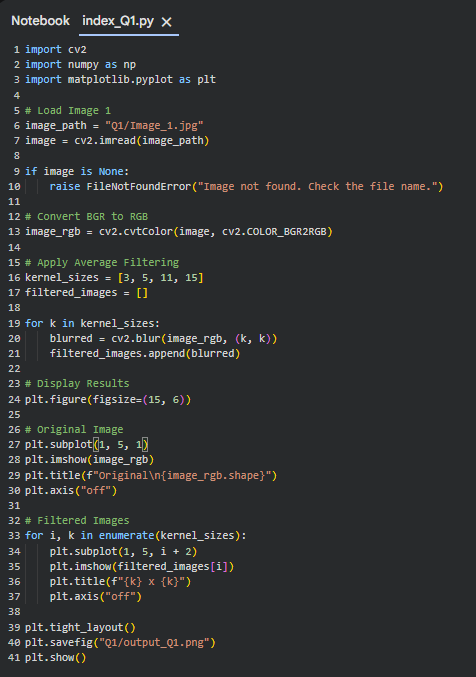
\includegraphics[width=0.85\textwidth]{Q1_code.png}
    \caption{Python implementation of average filtering with different kernel sizes}
\end{figure}


\subsubsection*{Results}

\begin{figure}[H]
    \centering
    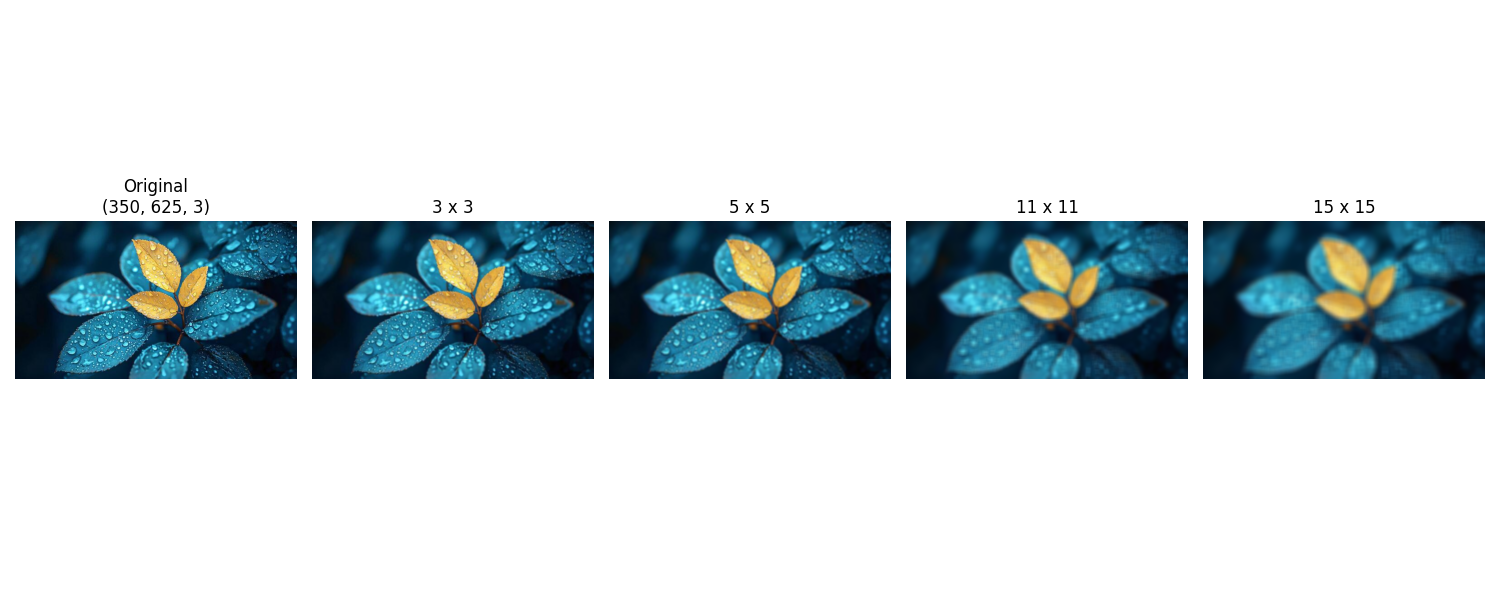
\includegraphics[width=0.85\textwidth]{output_Q1.png}
    \caption{Average filtering results using 3×3, 5×5, 11×11 and 15×15 kernels}
\end{figure}


\subsubsection*{Discussion and Observations}

Average filtering is a linear smoothing technique that replaces each pixel value with the mean of its neighboring pixels defined by the kernel window. As the kernel size increases from 3×3 to 15×15, the smoothing effect becomes progressively stronger. Smaller kernels slightly reduce noise while preserving most edge information. Larger kernels significantly blur the image, reduce sharp intensity transitions, and remove fine textures. Therefore, increasing the kernel size improves noise suppression but results in greater loss of edge sharpness and image details.

\hyperref[contents]{\small Back to Table of Contents}
\subsection{Question 2}

\subsubsection*{Objective}

Salt and pepper noise was added to Image 2 at 10\% and 20\% noise levels. 
Median filtering was then applied using kernel sizes 3×3, 5×5, and 11×11 to analyze the effect of increasing the kernel size on noise removal.


\subsubsection*{Code Snapshot}

\begin{figure}[H]
    \centering
    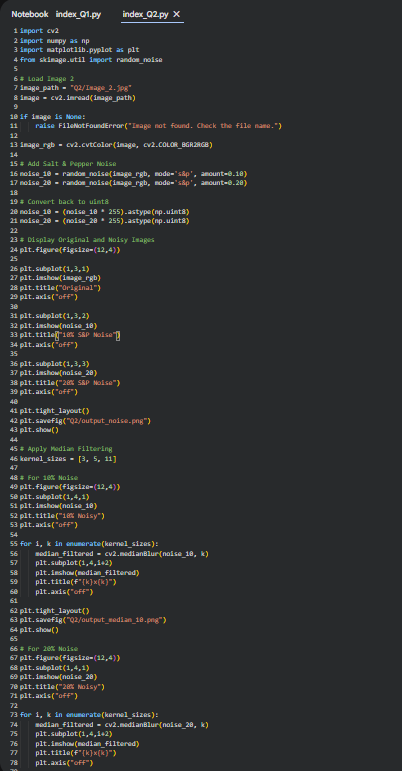
\includegraphics[width=0.85\textwidth]{Q2_code.png}
    \caption{Python implementation for adding salt and pepper noise and applying median filtering}
\end{figure}


\subsubsection*{Results}

\begin{figure}[H]
    \centering
    \begin{tabular}{cc}
        \includegraphics[width=0.45\textwidth]{Image_2.jpg} &
        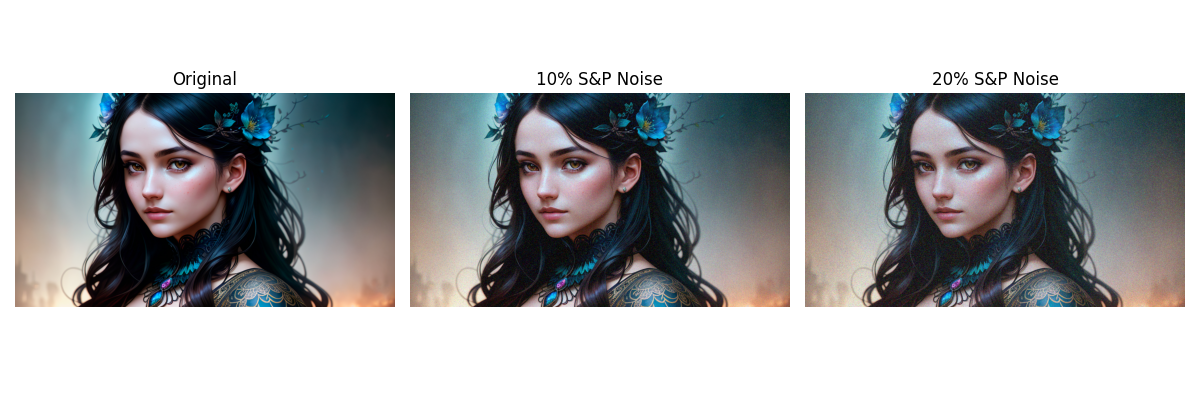
\includegraphics[width=0.45\textwidth]{output_noise.png} \\

        (a) Original Image &
        (b) Image with Salt and Pepper Noise \\[8pt]

        
\includegraphics[width=0.45\textwidth]{output_median_10.png} &
        
\includegraphics[width=0.45\textwidth]{output_median_20.png} \\

        (c) Median Filtering (10\% Noise) &
        (d) Median Filtering (20\% Noise)
    \end{tabular}
    \caption{Salt and pepper noise addition and median filtering results}
\end{figure}


\subsubsection*{Discussion and Observations}

Salt and pepper noise introduces random high and low intensity pixels in the image. 
Median filtering is a nonlinear smoothing technique that replaces each pixel with the median value of its neighborhood, making it highly effective for impulse noise removal.

For 10\% noise, smaller kernels such as 3×3 effectively remove most noisy pixels while preserving edge details. 
For 20\% noise, larger kernels such as 5×5 or 11×11 perform better in removing a higher density of noise but may slightly blur fine image structures.

Therefore, increasing the kernel size improves noise removal performance, but excessive kernel sizes reduce image sharpness and structural detail.

\hyperref[contents]{\small Back to Table of Contents}
\subsection{Question 3}

\subsubsection*{Objective}

Gaussian filtering was applied to Image 3 using kernel sizes 3×3, 5×5, 11×11, and 15×15. 
Additionally, the effect of varying the standard deviation $\sigma$ was analyzed for one selected kernel size.


\subsubsection*{Code Snapshot}

\begin{figure}[H]
    \centering
    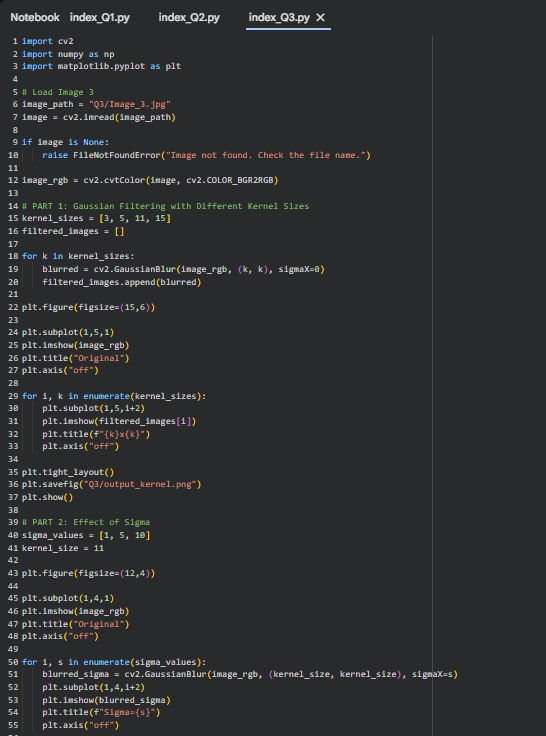
\includegraphics[width=0.85\textwidth]{Q3_code.png}
    \caption{Python implementation of Gaussian filtering with different kernel sizes and sigma values}
\end{figure}


\subsubsection*{Results}

\begin{figure}[H]
    \centering
    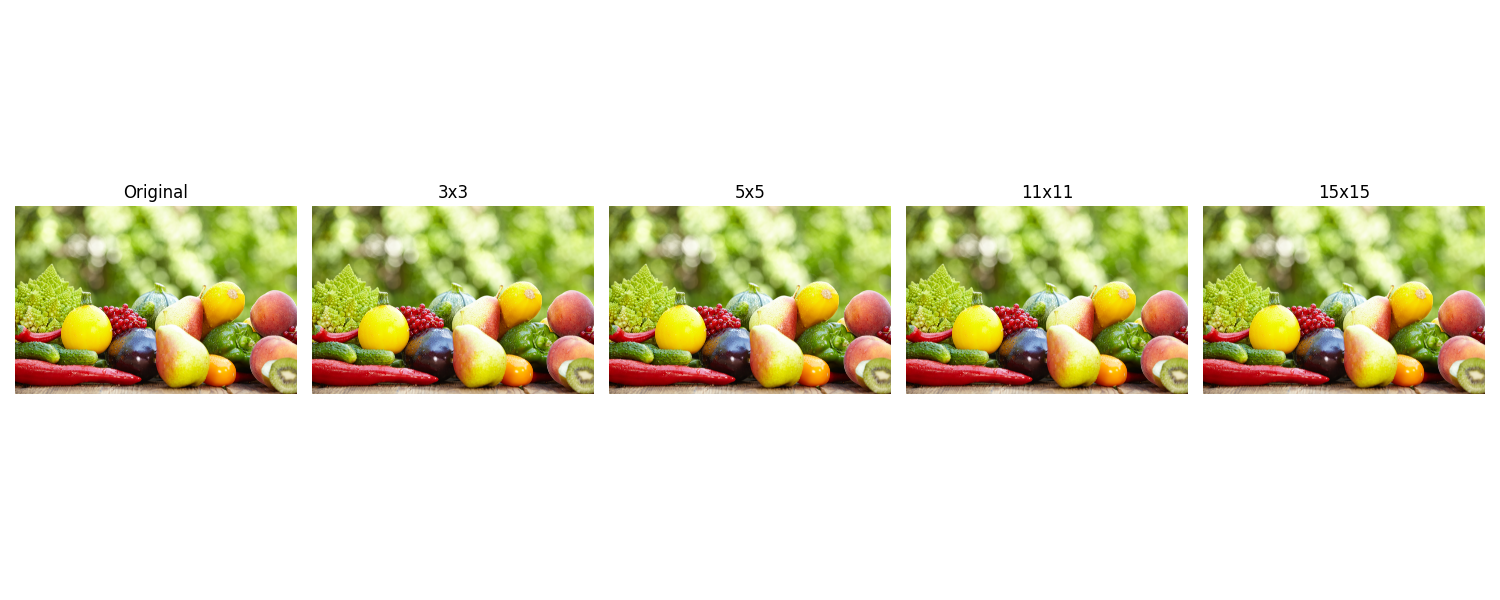
\includegraphics[width=0.85\textwidth]{output_kernel.png}
    \caption{Gaussian filtering results using kernel sizes 3×3, 5×5, 11×11 and 15×15}
\end{figure}

\begin{figure}[H]
    \centering
    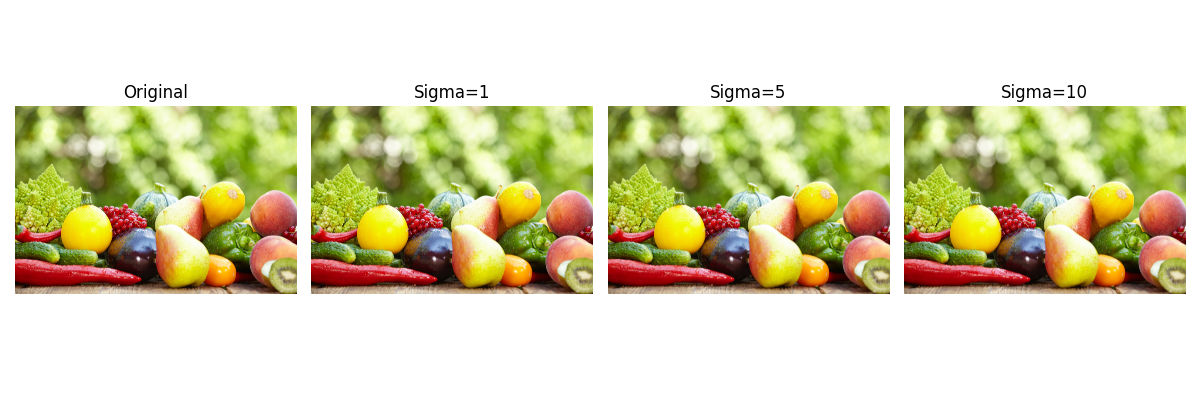
\includegraphics[width=0.85\textwidth]{output_sigma.png}
    \caption{Effect of varying standard deviation $\sigma$ in Gaussian filtering}
\end{figure}


\subsubsection*{Discussion and Observations}

Gaussian filtering is a weighted smoothing technique where neighboring pixels contribute according to a Gaussian distribution. 
As the kernel size increases, the smoothing effect becomes stronger and the image appears more blurred. Small kernels preserve more detail, while larger kernels reduce high frequency components and fine textures.

The standard deviation $\sigma$ controls the spread of the Gaussian function. A small $\sigma$ results in slight smoothing, while a larger $\sigma$ produces stronger blurring even if the kernel size remains constant. Therefore, both kernel size and $\sigma$ influence the degree of smoothing, with larger values leading to greater reduction of image detail and noise.

\hyperref[contents]{\small Back to Table of Contents}
\subsection{Question 4}

\subsubsection*{Objective}

A 3 level Gaussian pyramid and a 3 level Laplacian pyramid were generated for Image 4. 
An appropriate kernel size was selected to ensure smooth downsampling and proper reconstruction.


\subsubsection*{Code Snapshot}

\begin{figure}[H]
    \centering
    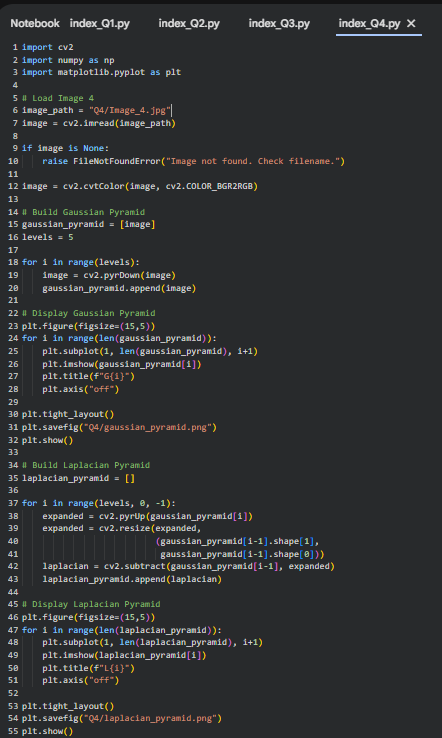
\includegraphics[width=0.85\textwidth]{Q4_code.png}
    \caption{Python implementation for generating Gaussian and Laplacian pyramids}
\end{figure}


\subsubsection*{Results}

\begin{figure}[H]
    \centering
    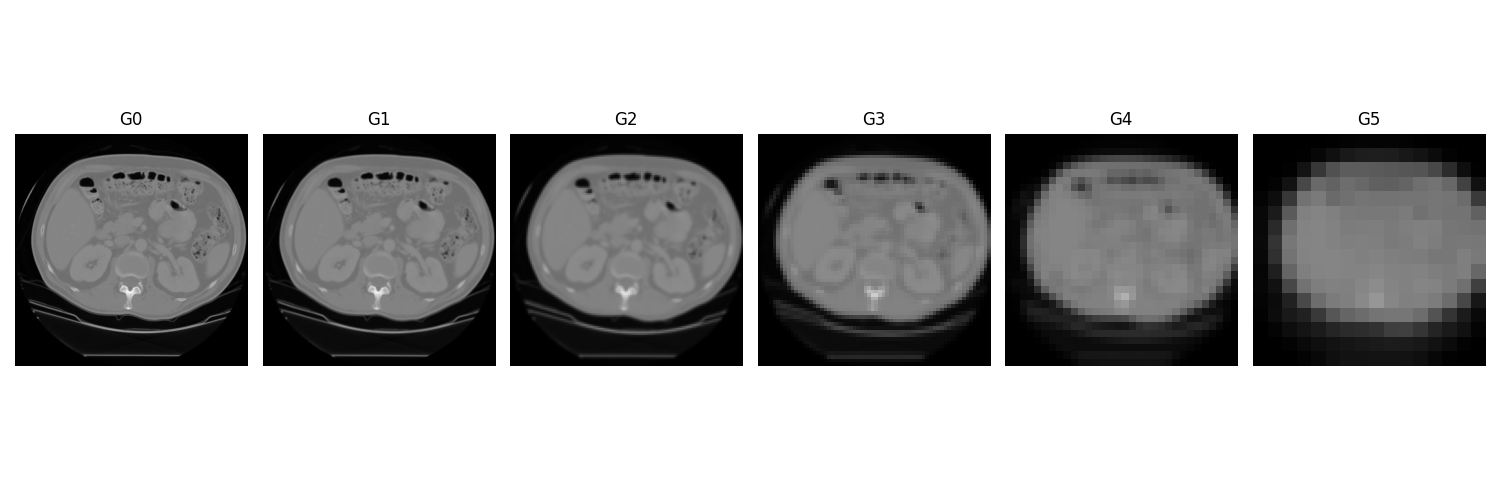
\includegraphics[width=0.85\textwidth]{gaussian_pyramid.png}
    \caption{Three level Gaussian pyramid}
\end{figure}

\begin{figure}[H]
    \centering
    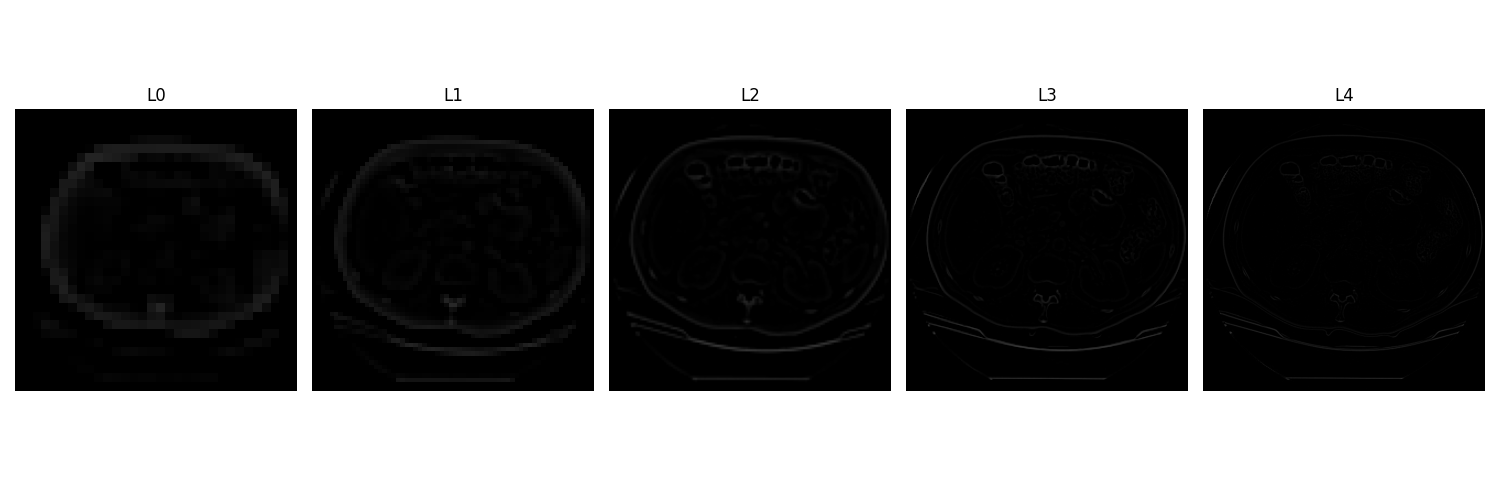
\includegraphics[width=0.85\textwidth]{laplacian_pyramid.png}
    \caption{Three level Laplacian pyramid}
\end{figure}


\subsubsection*{Discussion and Observations}

The Gaussian pyramid is constructed by repeatedly smoothing and downsampling the image, resulting in progressively lower resolution representations. 
A moderate Gaussian kernel (typically 5×5) was selected to ensure sufficient smoothing before downsampling, which prevents aliasing artifacts.

The Laplacian pyramid is obtained by subtracting consecutive Gaussian levels, capturing high frequency details such as edges and fine textures. 
Higher pyramid levels contain coarse structural information, while lower levels retain finer image details. 
The chosen kernel size ensures smooth transitions between pyramid levels and stable reconstruction.

\hyperref[contents]{\small Back to Table of Contents}
\subsection{Question 5}

\subsubsection*{Objective}

The largest kernel size from Question 1 (15×15 average filter) was implemented manually and compared with the OpenCV built in function. The difference image (A, B) was computed to analyze any variations.


\subsubsection*{Code Snapshot}

\begin{figure}[H]
    \centering
    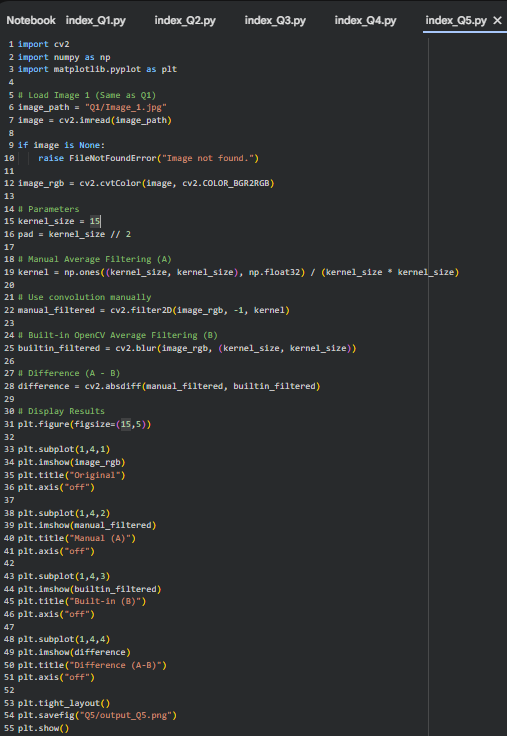
\includegraphics[width=0.85\textwidth]{Q5_code.png}
    \caption{Manual and built in average filtering comparison}
\end{figure}


\subsubsection*{Results}

\begin{figure}[H]
    \centering
    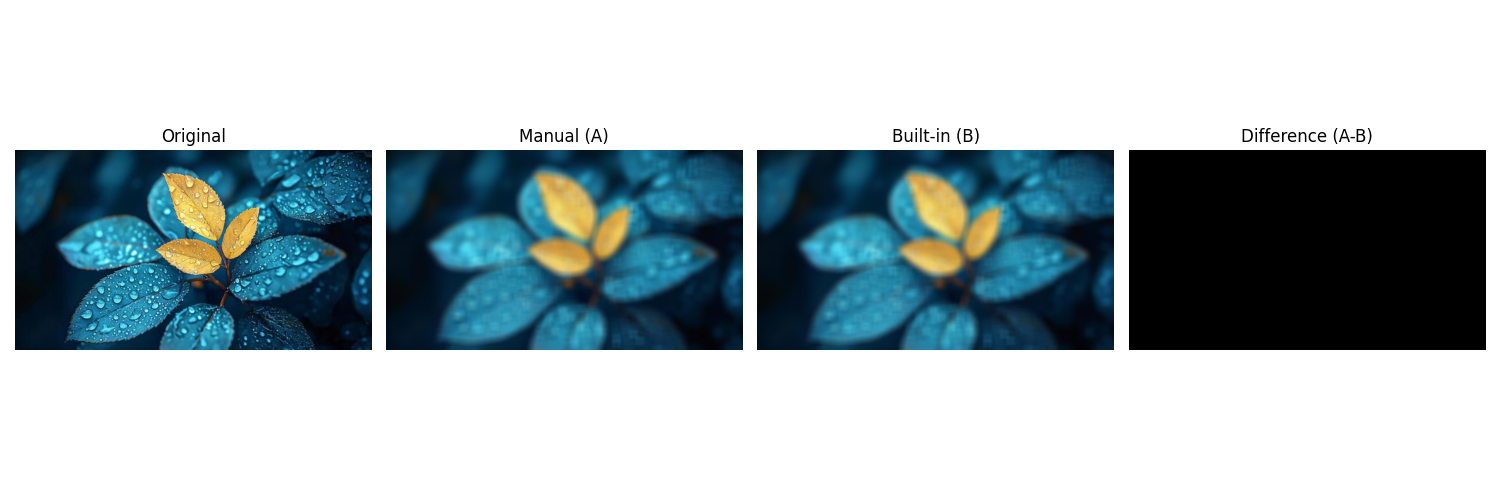
\includegraphics[width=0.85\textwidth]{output_Q5.png}
    \caption{Comparison of manual filtering (A), built in filtering (B), and their difference}
\end{figure}


\subsubsection*{Discussion and Observations}

The manual implementation and the OpenCV built in function produced nearly identical results. The difference image (A,B) appears almost black, indicating minimal variation between the two methods. Small differences may occur due to floating point rounding and border handling mechanisms used internally by OpenCV. Overall, both implementations perform equivalent average filtering operations.

\hyperref[contents]{\small Back to Table of Contents}
\subsection{Question 6}

\subsubsection*{Objective}

Let Image 3 be denoted as \( I \). The following operation was performed:

\[
I' = I + SP + L(I)
\]

where \( SP \) represents salt and pepper noise and \( L(I) \) is the Laplacian filtered output of the image. Wavelet decomposition was then applied using the Haar wavelet. High frequency components were removed, and the image was reconstructed to obtain a smoother version.


\subsubsection*{Code Snapshot}

\begin{figure}[H]
    \centering
    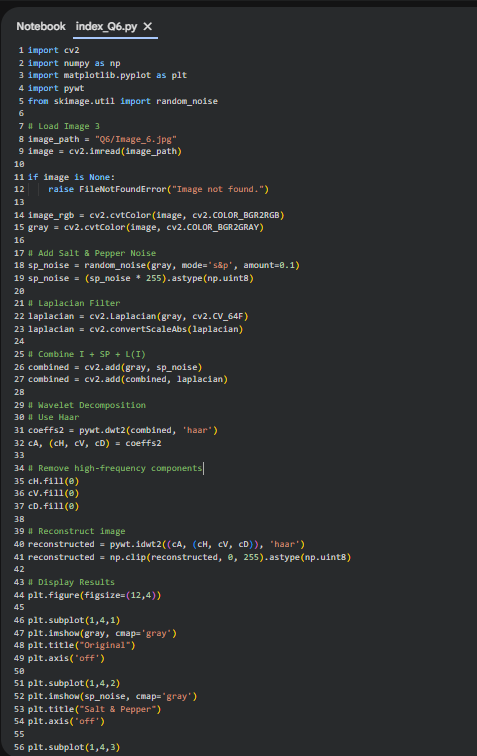
\includegraphics[width=0.85\textwidth]{Q6_code.png}
    \caption{Wavelet decomposition and reconstruction process}
\end{figure}


\subsubsection*{Results}

\begin{figure}[H]
    \centering
    
\includegraphics[width=0.85\textwidth]{wavelet_output.png}
    \caption{Wavelet decomposition result and reconstructed smooth image}
\end{figure}


\subsubsection*{Discussion and Observations}

The modified image \( I' \) contains both impulse noise and enhanced edge components due to the Laplacian operation. Wavelet decomposition separates the image into low frequency (approximation) and high frequency (detail) components. By removing or suppressing the high frequency sub bands and reconstructing the image, a smoother image is obtained. The reconstructed image shows reduced noise and reduced sharp edge intensity compared to the original noisy image, demonstrating the effectiveness of wavelet based denoising.

\hyperref[contents]{\small Back to Table of Contents}
\subsection{Question 7}

\subsubsection*{Objective}

Digital watermarking was performed on Image 3 using the Discrete Wavelet Transform (DWT). The watermark was embedded in the frequency domain and later extracted to verify successful embedding.


\subsubsection*{Code Snapshot}

\begin{figure}[H]
    \centering
    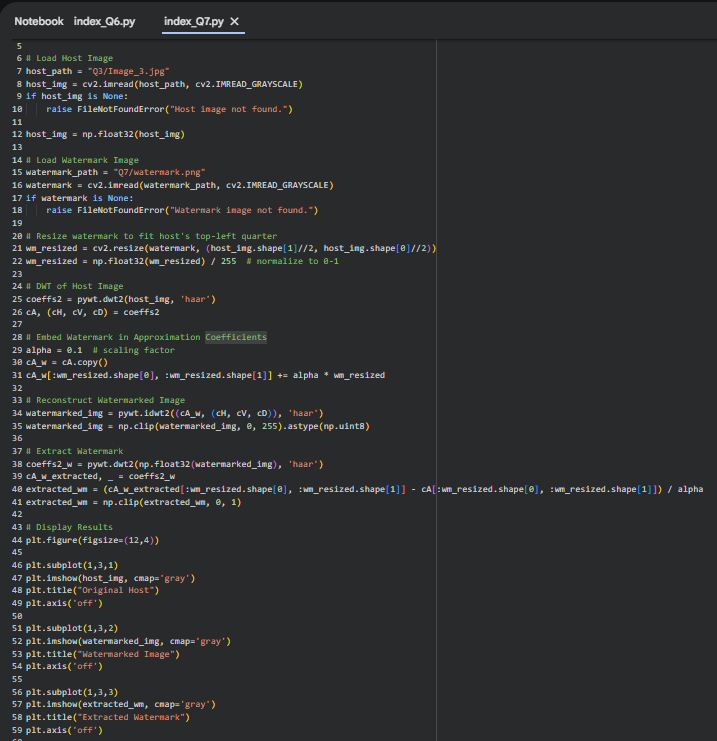
\includegraphics[width=0.85\textwidth]{Q7_code.png}
    \caption{DWT based watermark embedding and extraction process}
\end{figure}


\subsubsection*{Results}

\begin{figure}[H]
    \centering
    \begin{tabular}{cc}
        
\includegraphics[width=0.40\textwidth]{watermark.png} &
        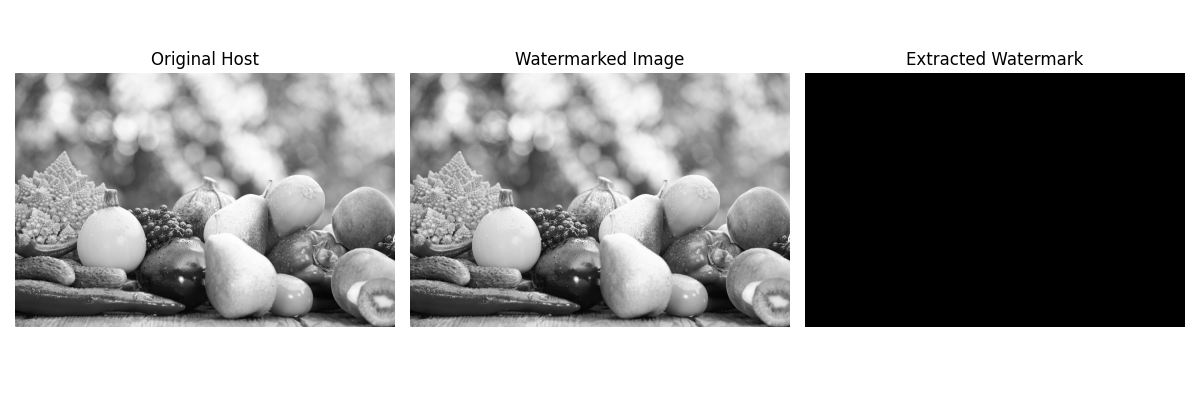
\includegraphics[width=0.40\textwidth]{watermark_output.png} \\

        (a) Original Watermark &
        (b) Watermarked and Extracted Result
    \end{tabular}
    \caption{Digital watermark embedding and extraction using DWT}
\end{figure}


\subsubsection*{Discussion and Observations}

The Discrete Wavelet Transform decomposes the image into four sub bands: LL, LH, HL, and HH. The watermark was embedded into one of the high frequency sub bands to ensure minimal perceptual distortion of the host image. Embedding in the frequency domain improves robustness compared to spatial domain methods.

After applying the inverse wavelet transform, the watermarked image retained visual quality while containing the hidden watermark. During extraction, the watermark was successfully recovered, demonstrating that DWT based watermarking provides a balance between imperceptibility and robustness.

\hyperref[contents]{\small Back to Table of Contents}
\subsection{Question 8}

\subsubsection*{Objective}

The organs of interest were extracted from the provided CT image using classical image segmentation techniques. Intensity based thresholding and morphological operations were applied to isolate the required anatomical structures.


\subsubsection*{Code Snapshot}

\begin{figure}[H]
    \centering
    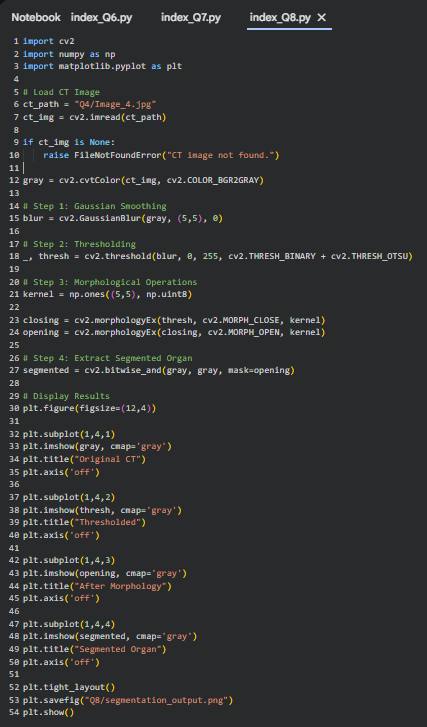
\includegraphics[width=0.85\textwidth]{Q8_code.png}
    \caption{CT image segmentation using thresholding and morphological operations}
\end{figure}


\subsubsection*{Results}

\begin{figure}[H]
    \centering
    
\includegraphics[width=0.85\textwidth]{segmentation_output.png}
    \caption{Original CT image and segmented organs of interest}
\end{figure}


\subsubsection*{Discussion and Observations}

CT images represent tissues with different intensity values based on their density. The organs of interest were segmented by selecting an appropriate intensity threshold to separate them from surrounding tissues. Morphological operations such as erosion, dilation, opening, and closing were used to remove small artifacts and refine the segmented regions.

The final result successfully isolates the target organs while reducing noise and background interference. This demonstrates that classical intensity based segmentation combined with morphological processing can effectively extract anatomical structures in medical images.

\hyperref[contents]{\small Back to Table of Contents}
\subsection{Question 9}

\subsubsection*{Objective}

The provided MRI image was enhanced using three classical image enhancement techniques: histogram equalization, contrast stretching, and Gaussian filtering for noise reduction. The results were compared to determine the most suitable method for clinical diagnosis.


\subsubsection*{Code Snapshot}

\begin{figure}[H]
    \centering
    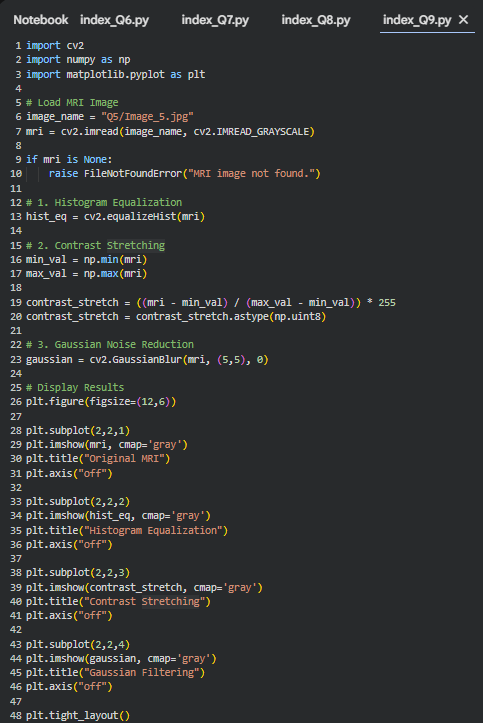
\includegraphics[width=0.85\textwidth]{Q9_code.png}
    \caption{MRI enhancement using histogram equalization, contrast stretching, and Gaussian filtering}
\end{figure}


\subsubsection*{Results}

\begin{figure}[H]
    \centering
    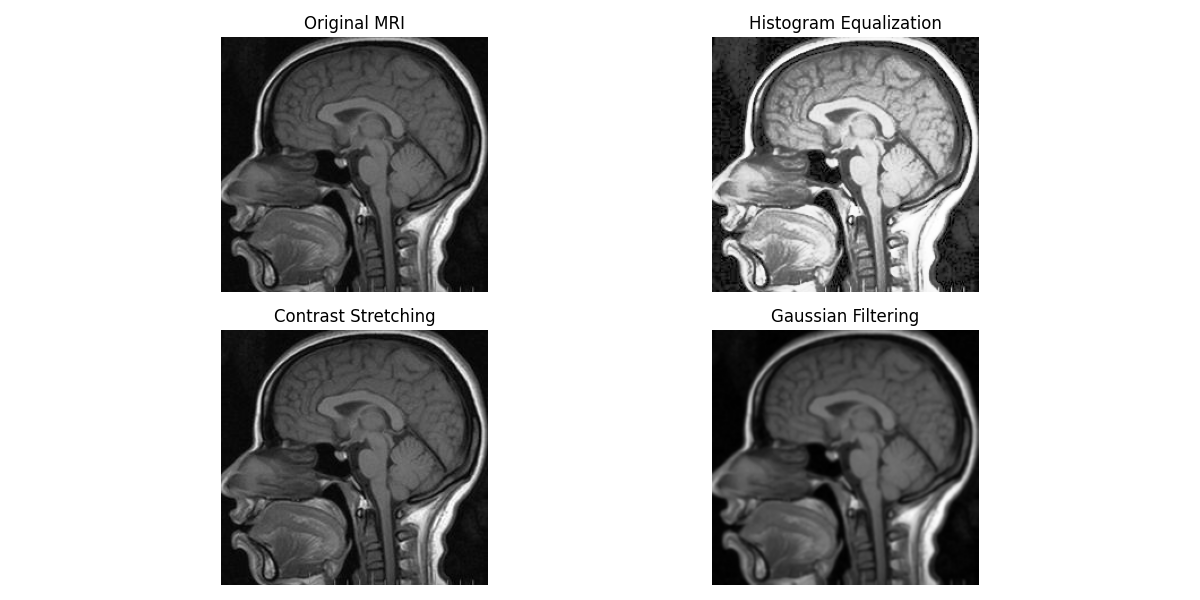
\includegraphics[width=0.85\textwidth]{mri_enhancement.png}
    \caption{Comparison of original MRI image and enhanced results}
\end{figure}


\subsubsection*{Discussion and Observations}

Histogram equalization enhances global contrast by redistributing intensity values, making structures more visible. However, it may amplify noise in uniform regions. Contrast stretching improves image visibility by expanding the intensity range without significantly increasing noise.

Gaussian filtering reduces noise by smoothing the image, but excessive smoothing may reduce fine anatomical details. For clinical diagnosis, contrast stretching provides a balanced improvement in visibility while preserving structural information. Histogram equalization enhances contrast more aggressively, while Gaussian filtering is mainly useful for noise suppression rather than contrast enhancement.

\hyperref[contents]{\small Back to Table of Contents}
\subsection{Question 10}

\subsubsection*{Objective}

Morphological image analysis was performed on the provided synthetic grayscale image containing geometric objects and noise. The image was converted into binary form and morphological operations including erosion, dilation, opening, and closing were applied. Basic morphological features such as area and perimeter were also extracted.


\subsubsection*{Code Snapshot}

\begin{figure}[H]
    \centering
    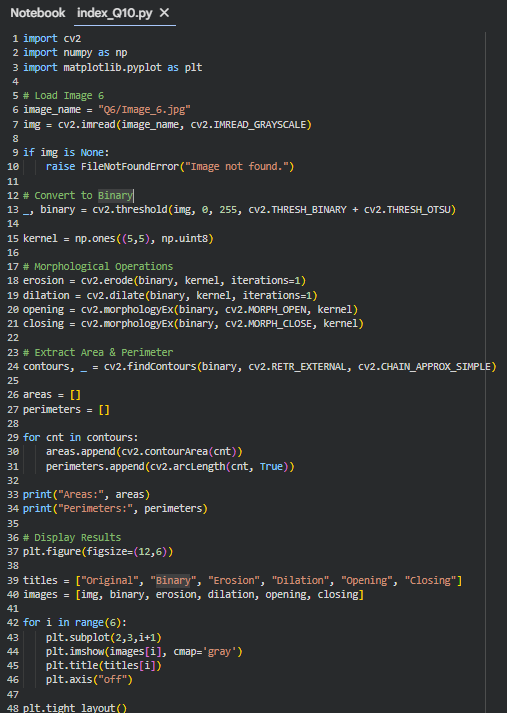
\includegraphics[width=0.85\textwidth]{Q10_code.png}
    \caption{Morphological operations and feature extraction implementation}
\end{figure}


\subsubsection*{Results}

\begin{figure}[H]
    \centering
    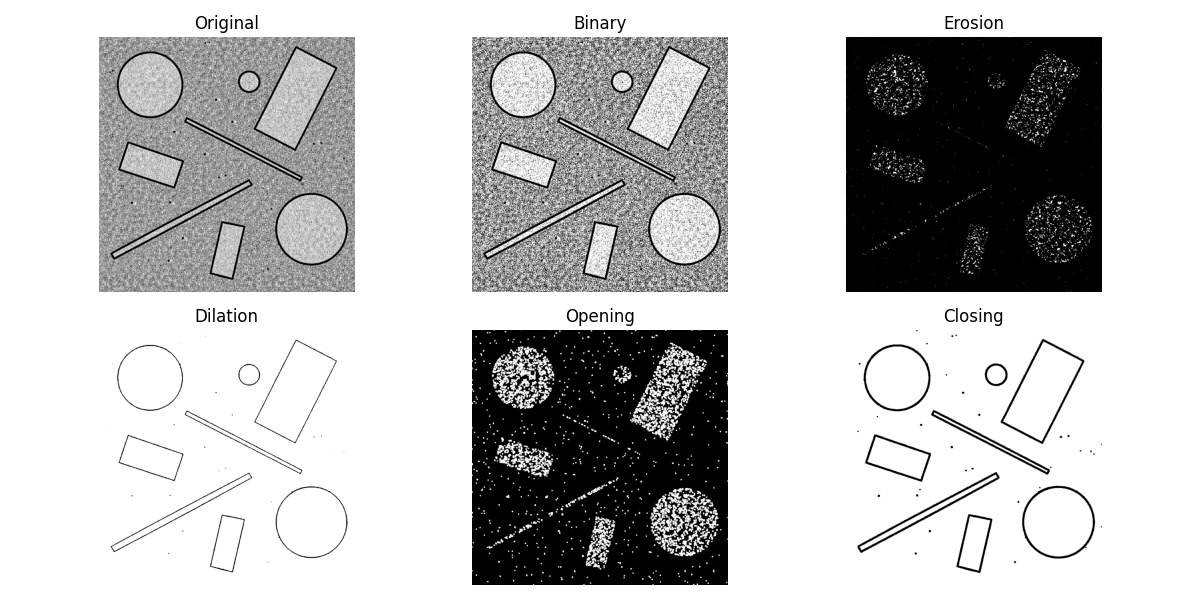
\includegraphics[width=0.85\textwidth]{morphological_results.png}
    \caption{Binary image and results of erosion, dilation, opening, and closing}
\end{figure}


\subsubsection*{Comparison of Morphological Operations}

\begin{table}[H]
\centering
\begin{tabular}{|c|c|c|c|}
\hline
Operation & Noise Removal & Gap Filling & Shape Preservation \\
\hline
Erosion & Removes small white noise & No & Shrinks objects \\
Dilation & Does not remove noise & Fills small gaps & Expands objects \\
Opening & Removes small noise & No & Preserves main shape \\
Closing & Reduces small holes & Fills gaps & Preserves object boundaries \\
\hline
\end{tabular}
\caption{Comparison of morphological operations}
\end{table}


\subsubsection*{Discussion and Observations}

Erosion reduces object boundaries and removes small white noise but shrinks object size. Dilation expands object boundaries and fills small gaps but may enlarge noise. Opening (erosion followed by dilation) effectively removes small noise while maintaining overall object structure. Closing (dilation followed by erosion) fills small holes and connects nearby components. 

Area and perimeter measurements were computed from the cleaned binary image, demonstrating how morphological operations assist in preparing images for quantitative shape analysis.


\hyperref[contents]{\small Back to Table of Contents}
\newpage


\section{Practical Work}

\subsection*{Introduction}

This practical task focuses on retinal vessel segmentation in fundus images using classical image processing techniques. A student-defined pipeline was developed using illumination correction, global thresholding, and morphological operations. The performance was evaluated quantitatively using Dice Similarity Coefficient and Jaccard Index on a validation subset.

\subsection*{Flow Diagram of the Image Processing Pipeline}

\begin{center}
\fbox{
\begin{minipage}{0.9\textwidth}
\centering

Input Fundus Image \\
$\downarrow$ \\
Green Channel Extraction \\
$\downarrow$ \\
Gaussian Blur (61×61) \\
$\downarrow$ \\
Illumination Correction \\
$\downarrow$ \\
Normalization \\
$\downarrow$ \\
Circular Masking \\
$\downarrow$ \\
Global Thresholding (T = 8) \\
$\downarrow$ \\
Dilation (2 Iterations) \\
$\downarrow$ \\
Morphological Closing \\
$\downarrow$ \\
Final Vessel Segmentation \\
$\downarrow$ \\
Performance Evaluation (Dice \& Jaccard)

\end{minipage}
}
\end{center}

\hyperref[contents]{\small Back to Table of Contents}
\newpage

\section*{Introduction and stepwise justification of the selected image processing pipeline.}

The green channel was extracted since retinal vessels exhibit higher contrast in this channel. A large Gaussian filter (61×61) was applied to estimate slow varying background illumination. Subtracting the blurred image enhanced vessel structures by emphasizing high frequency components. The corrected image was normalized and segmented using a low global threshold (T = 8) to preserve thin vessels. Morphological dilation (2 iterations) restored fragmented vessel segments, and closing was applied to connect discontinuities. This classical pipeline improves vessel visibility while suppressing background noise and illumination variations.

\hyperref[contents]{\small Back to Table of Contents}
\newpage

\section*{Expected Results for 10 Images}

\begin{figure}[H]
\centering
\renewcommand{\arraystretch}{1.2}
\begin{tabular}{ccc}

\textbf{Original} & \textbf{Segmented Result} & \textbf{Ground Truth} \\[8pt]


\includegraphics[width=0.28\textwidth]{training_set/images/1_A.png} &
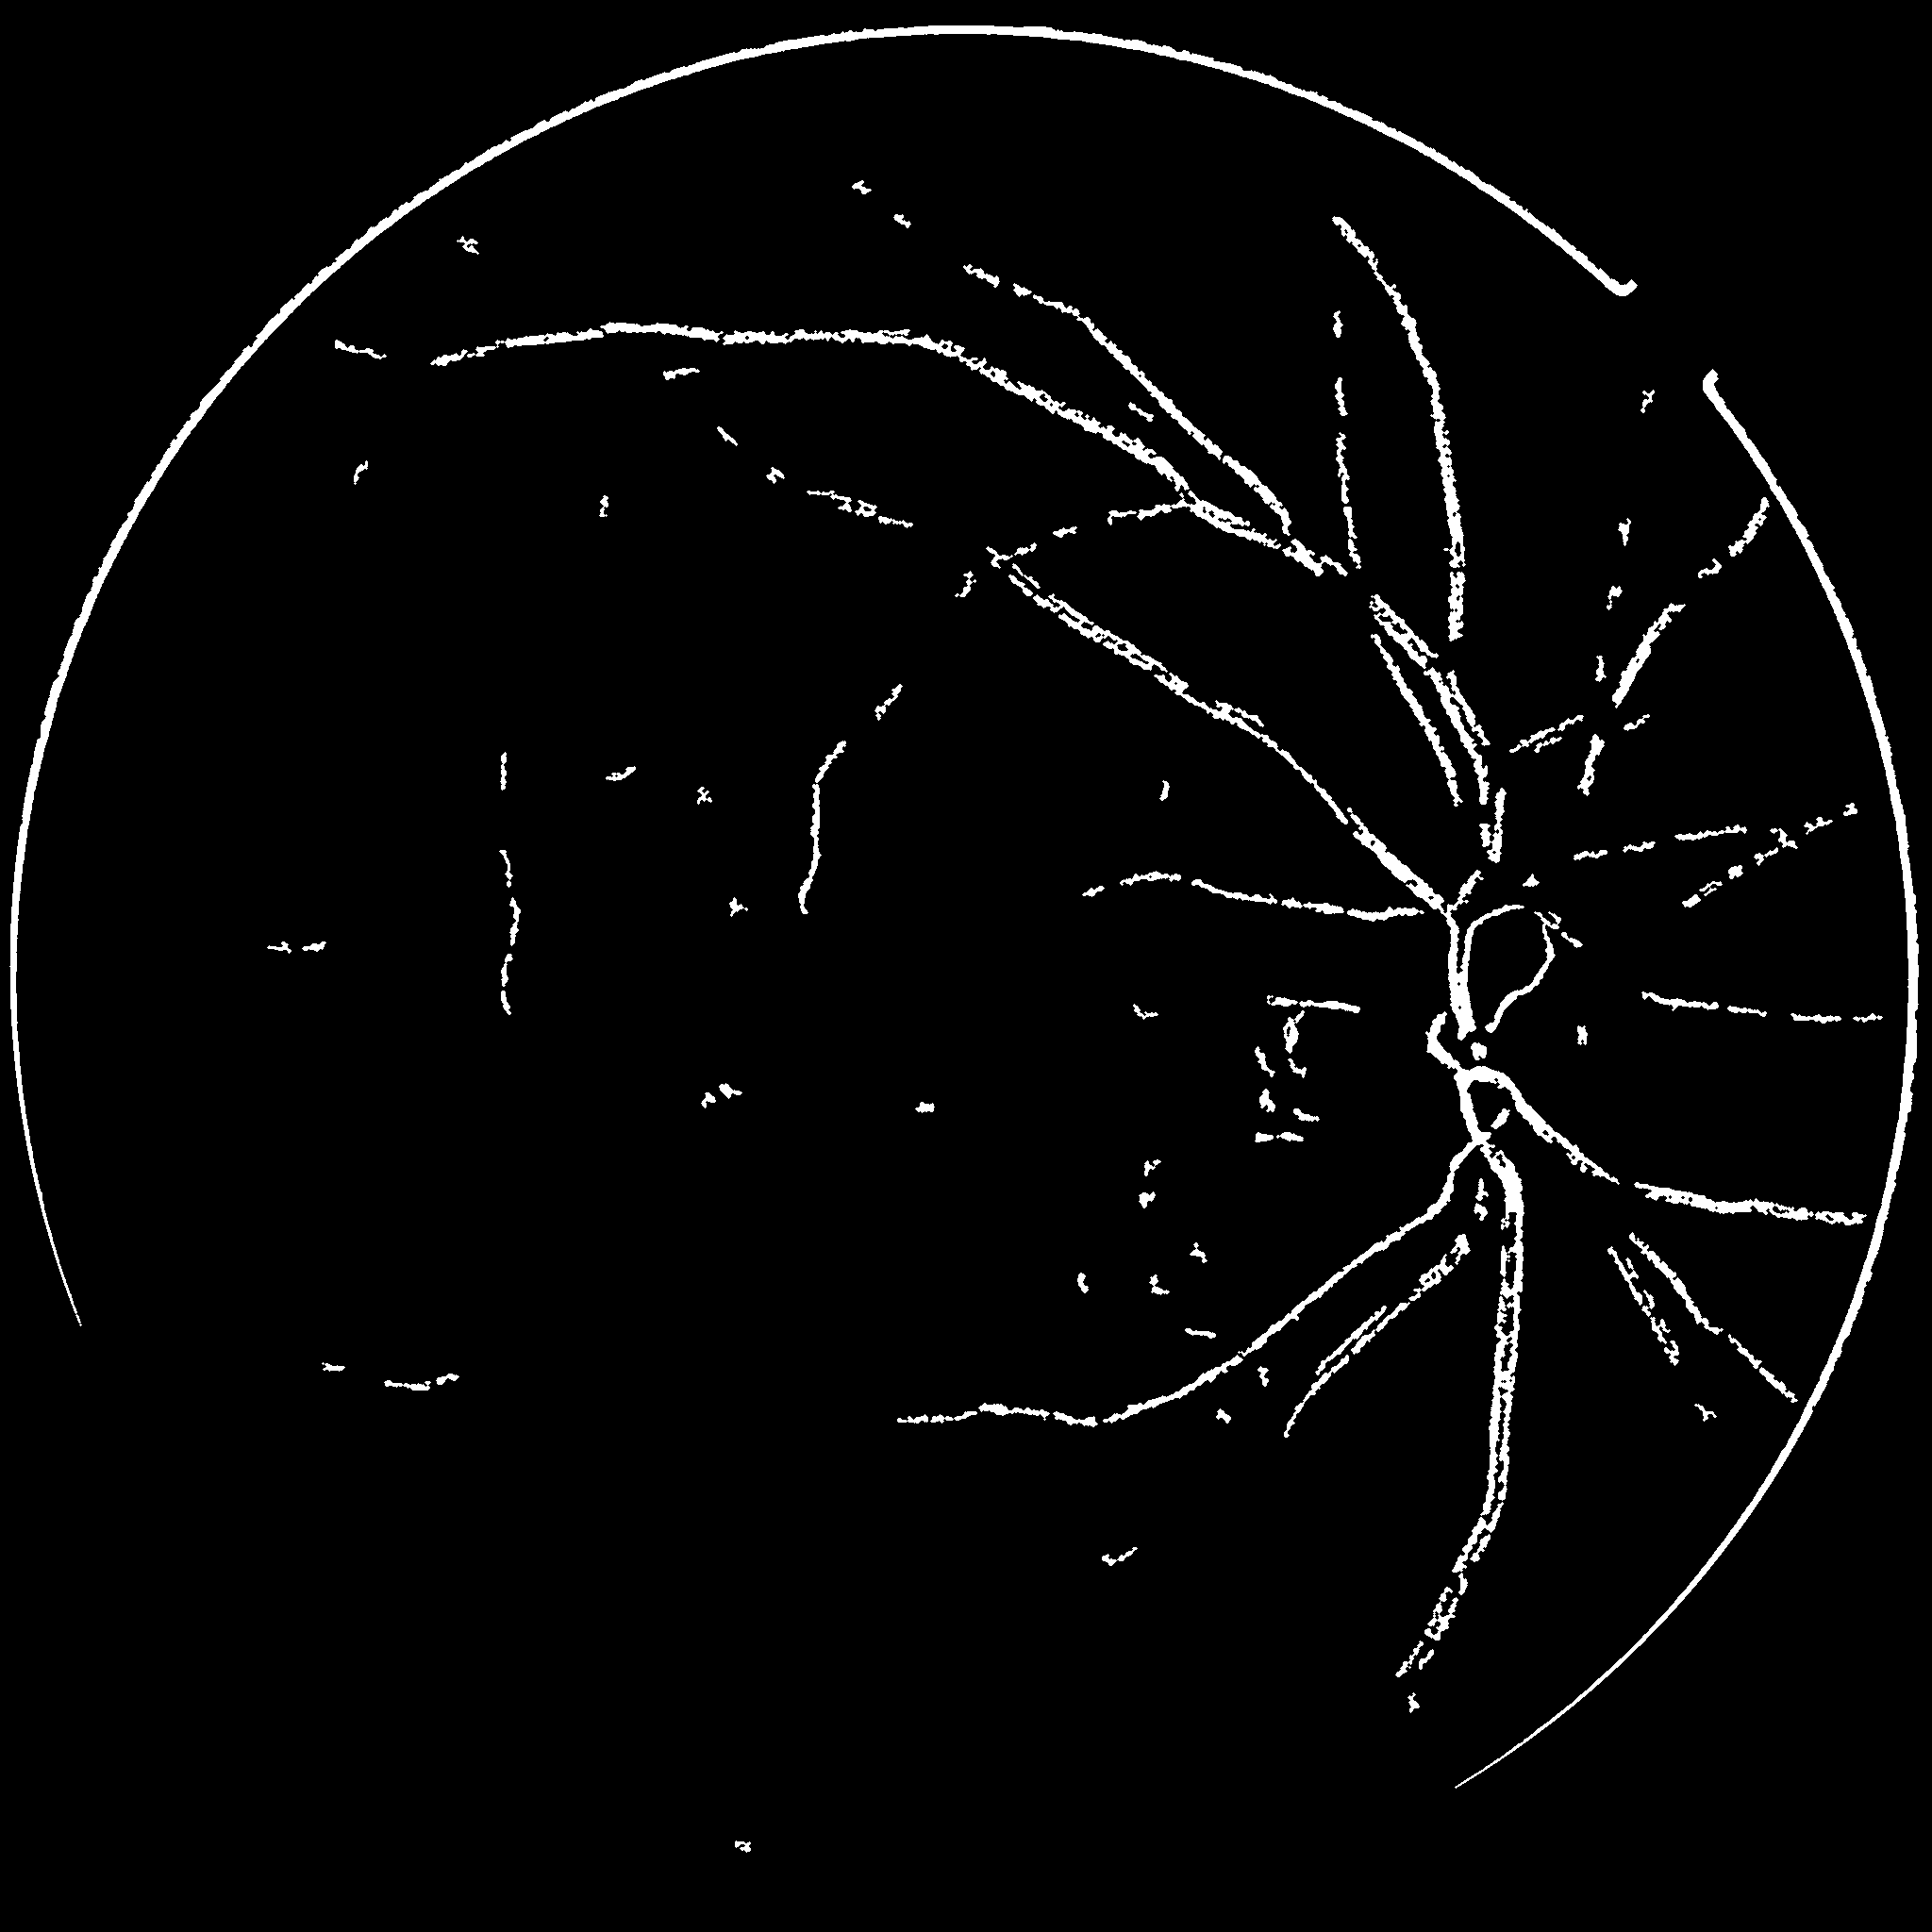
\includegraphics[width=0.28\textwidth]{results/1_A.png} &

\includegraphics[width=0.28\textwidth]{validation_set/masks/1_A.png} \\[10pt]


\includegraphics[width=0.28\textwidth]{training_set/images/2_A.png} &
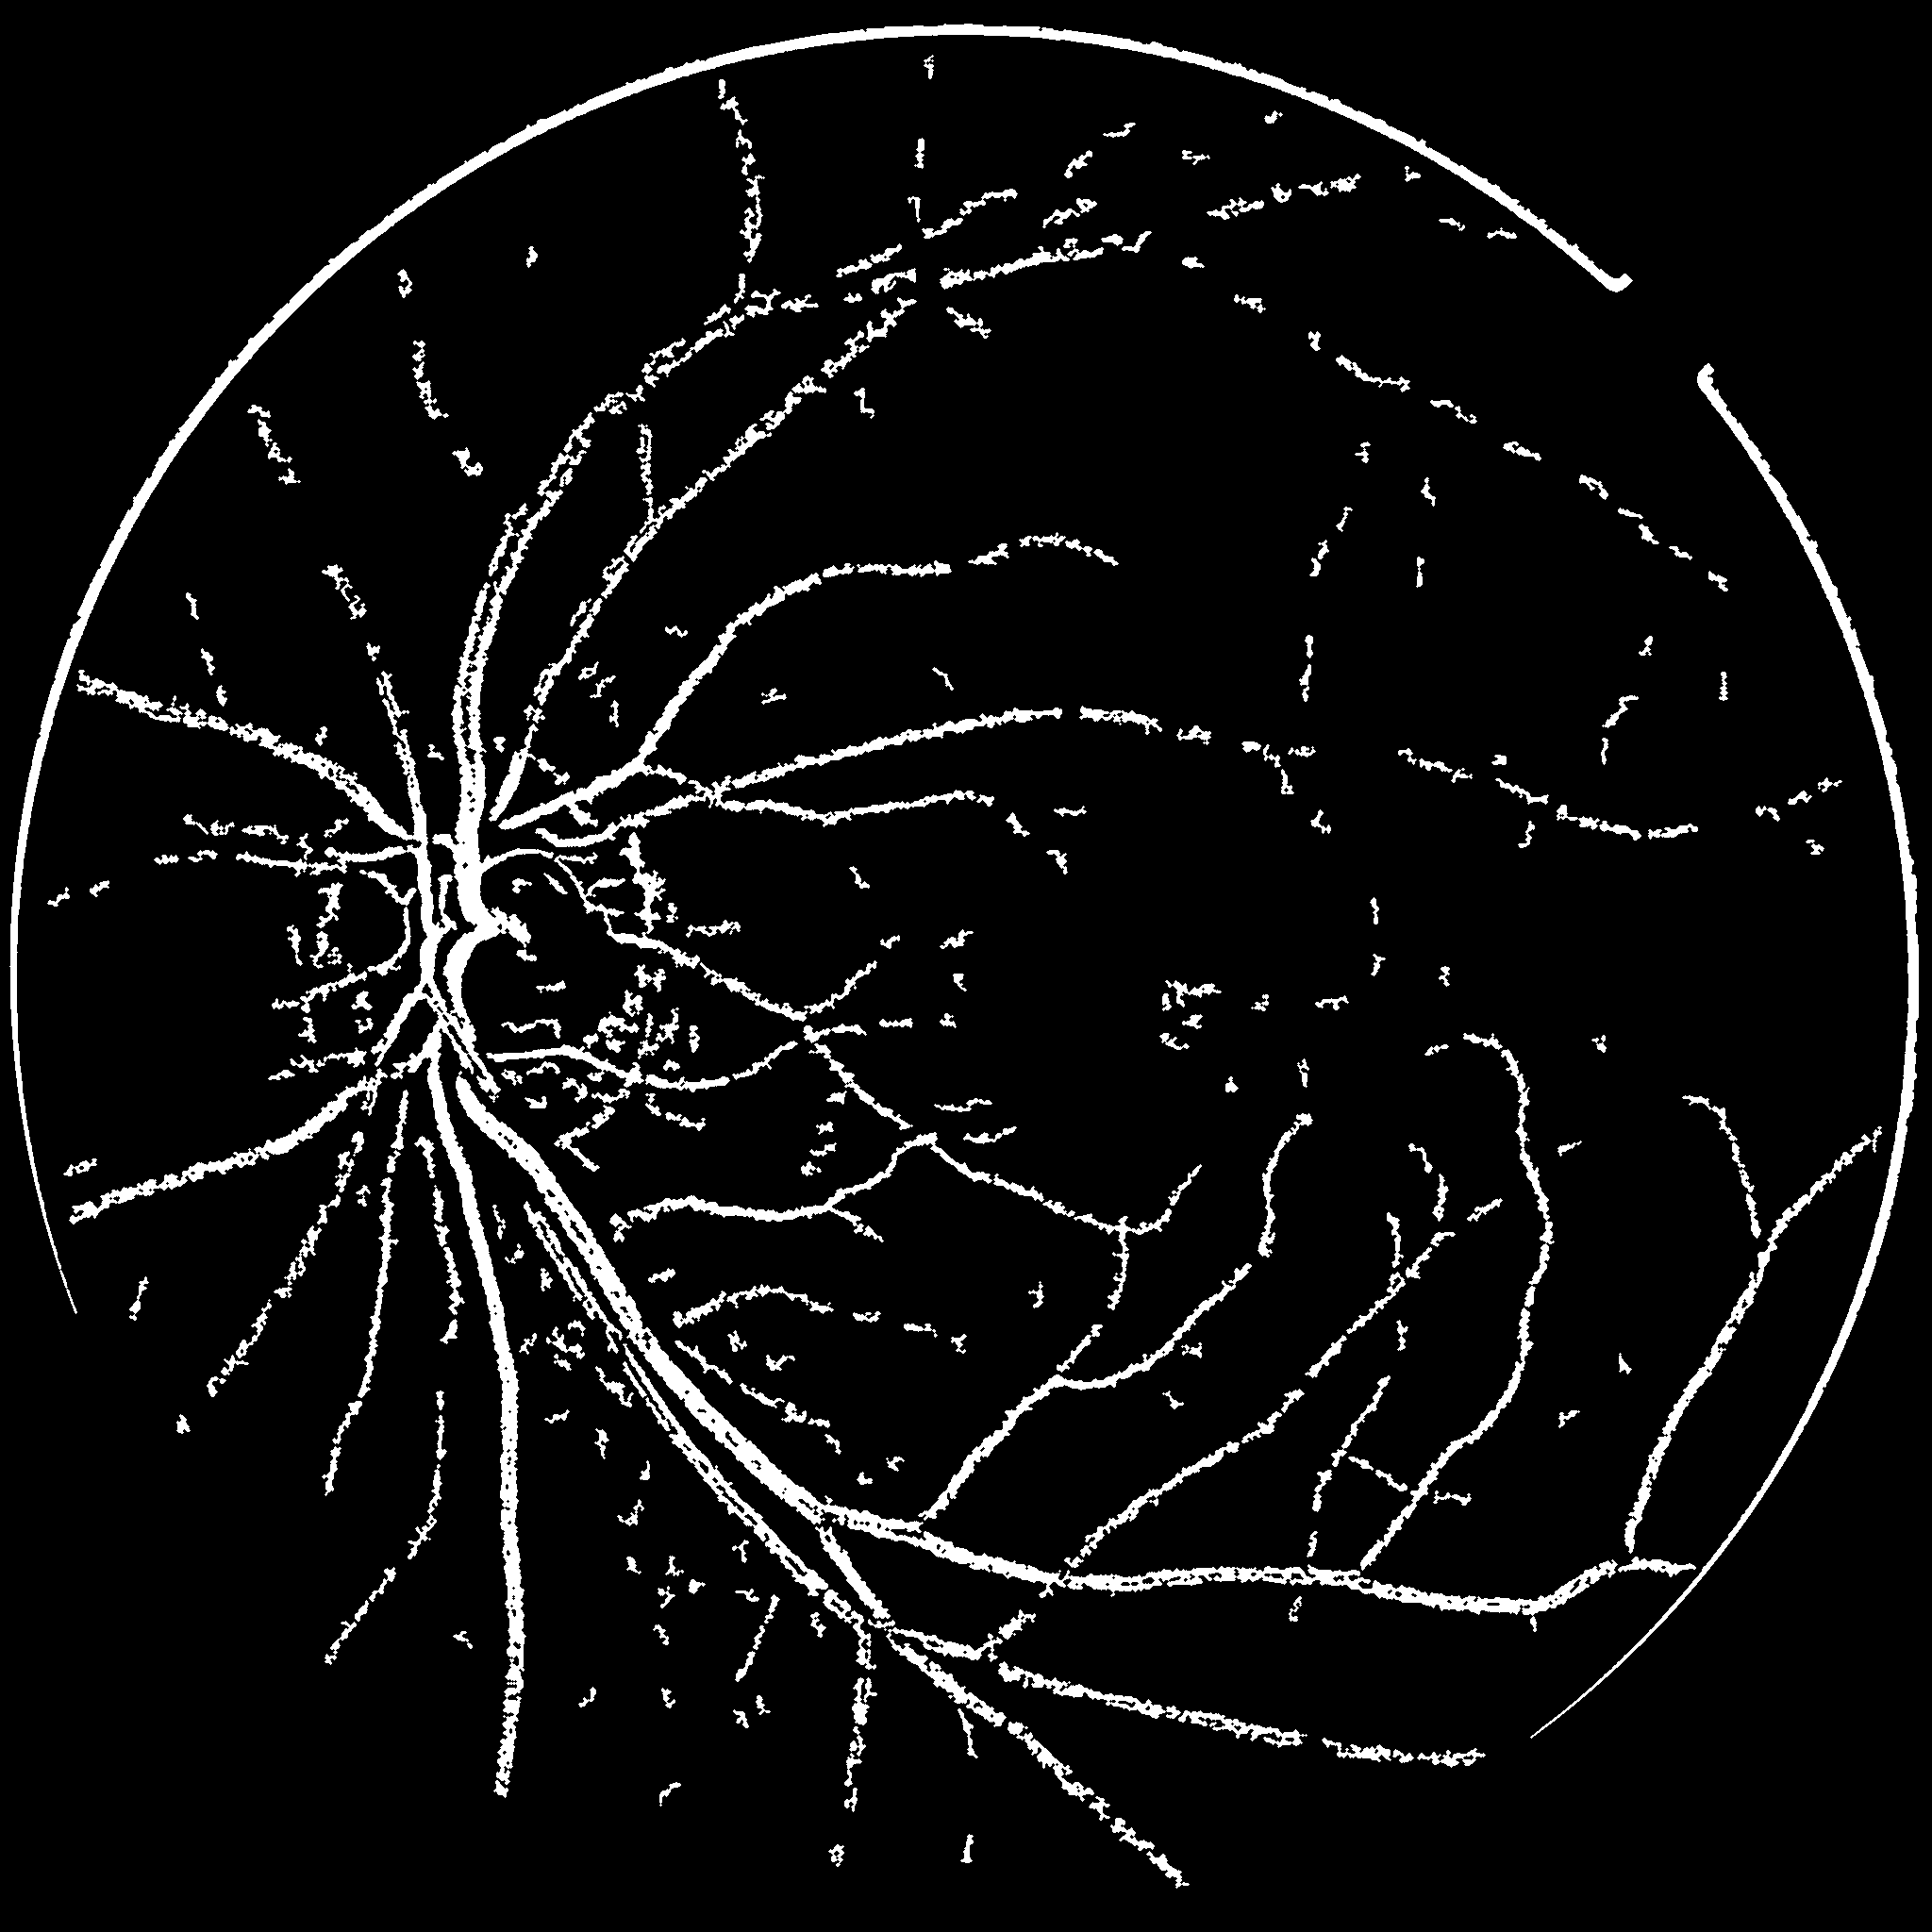
\includegraphics[width=0.28\textwidth]{results/2_A.png} &

\includegraphics[width=0.28\textwidth]{validation_set/masks/2_A.png} \\[10pt]


\includegraphics[width=0.28\textwidth]{training_set/images/3_A.png} &
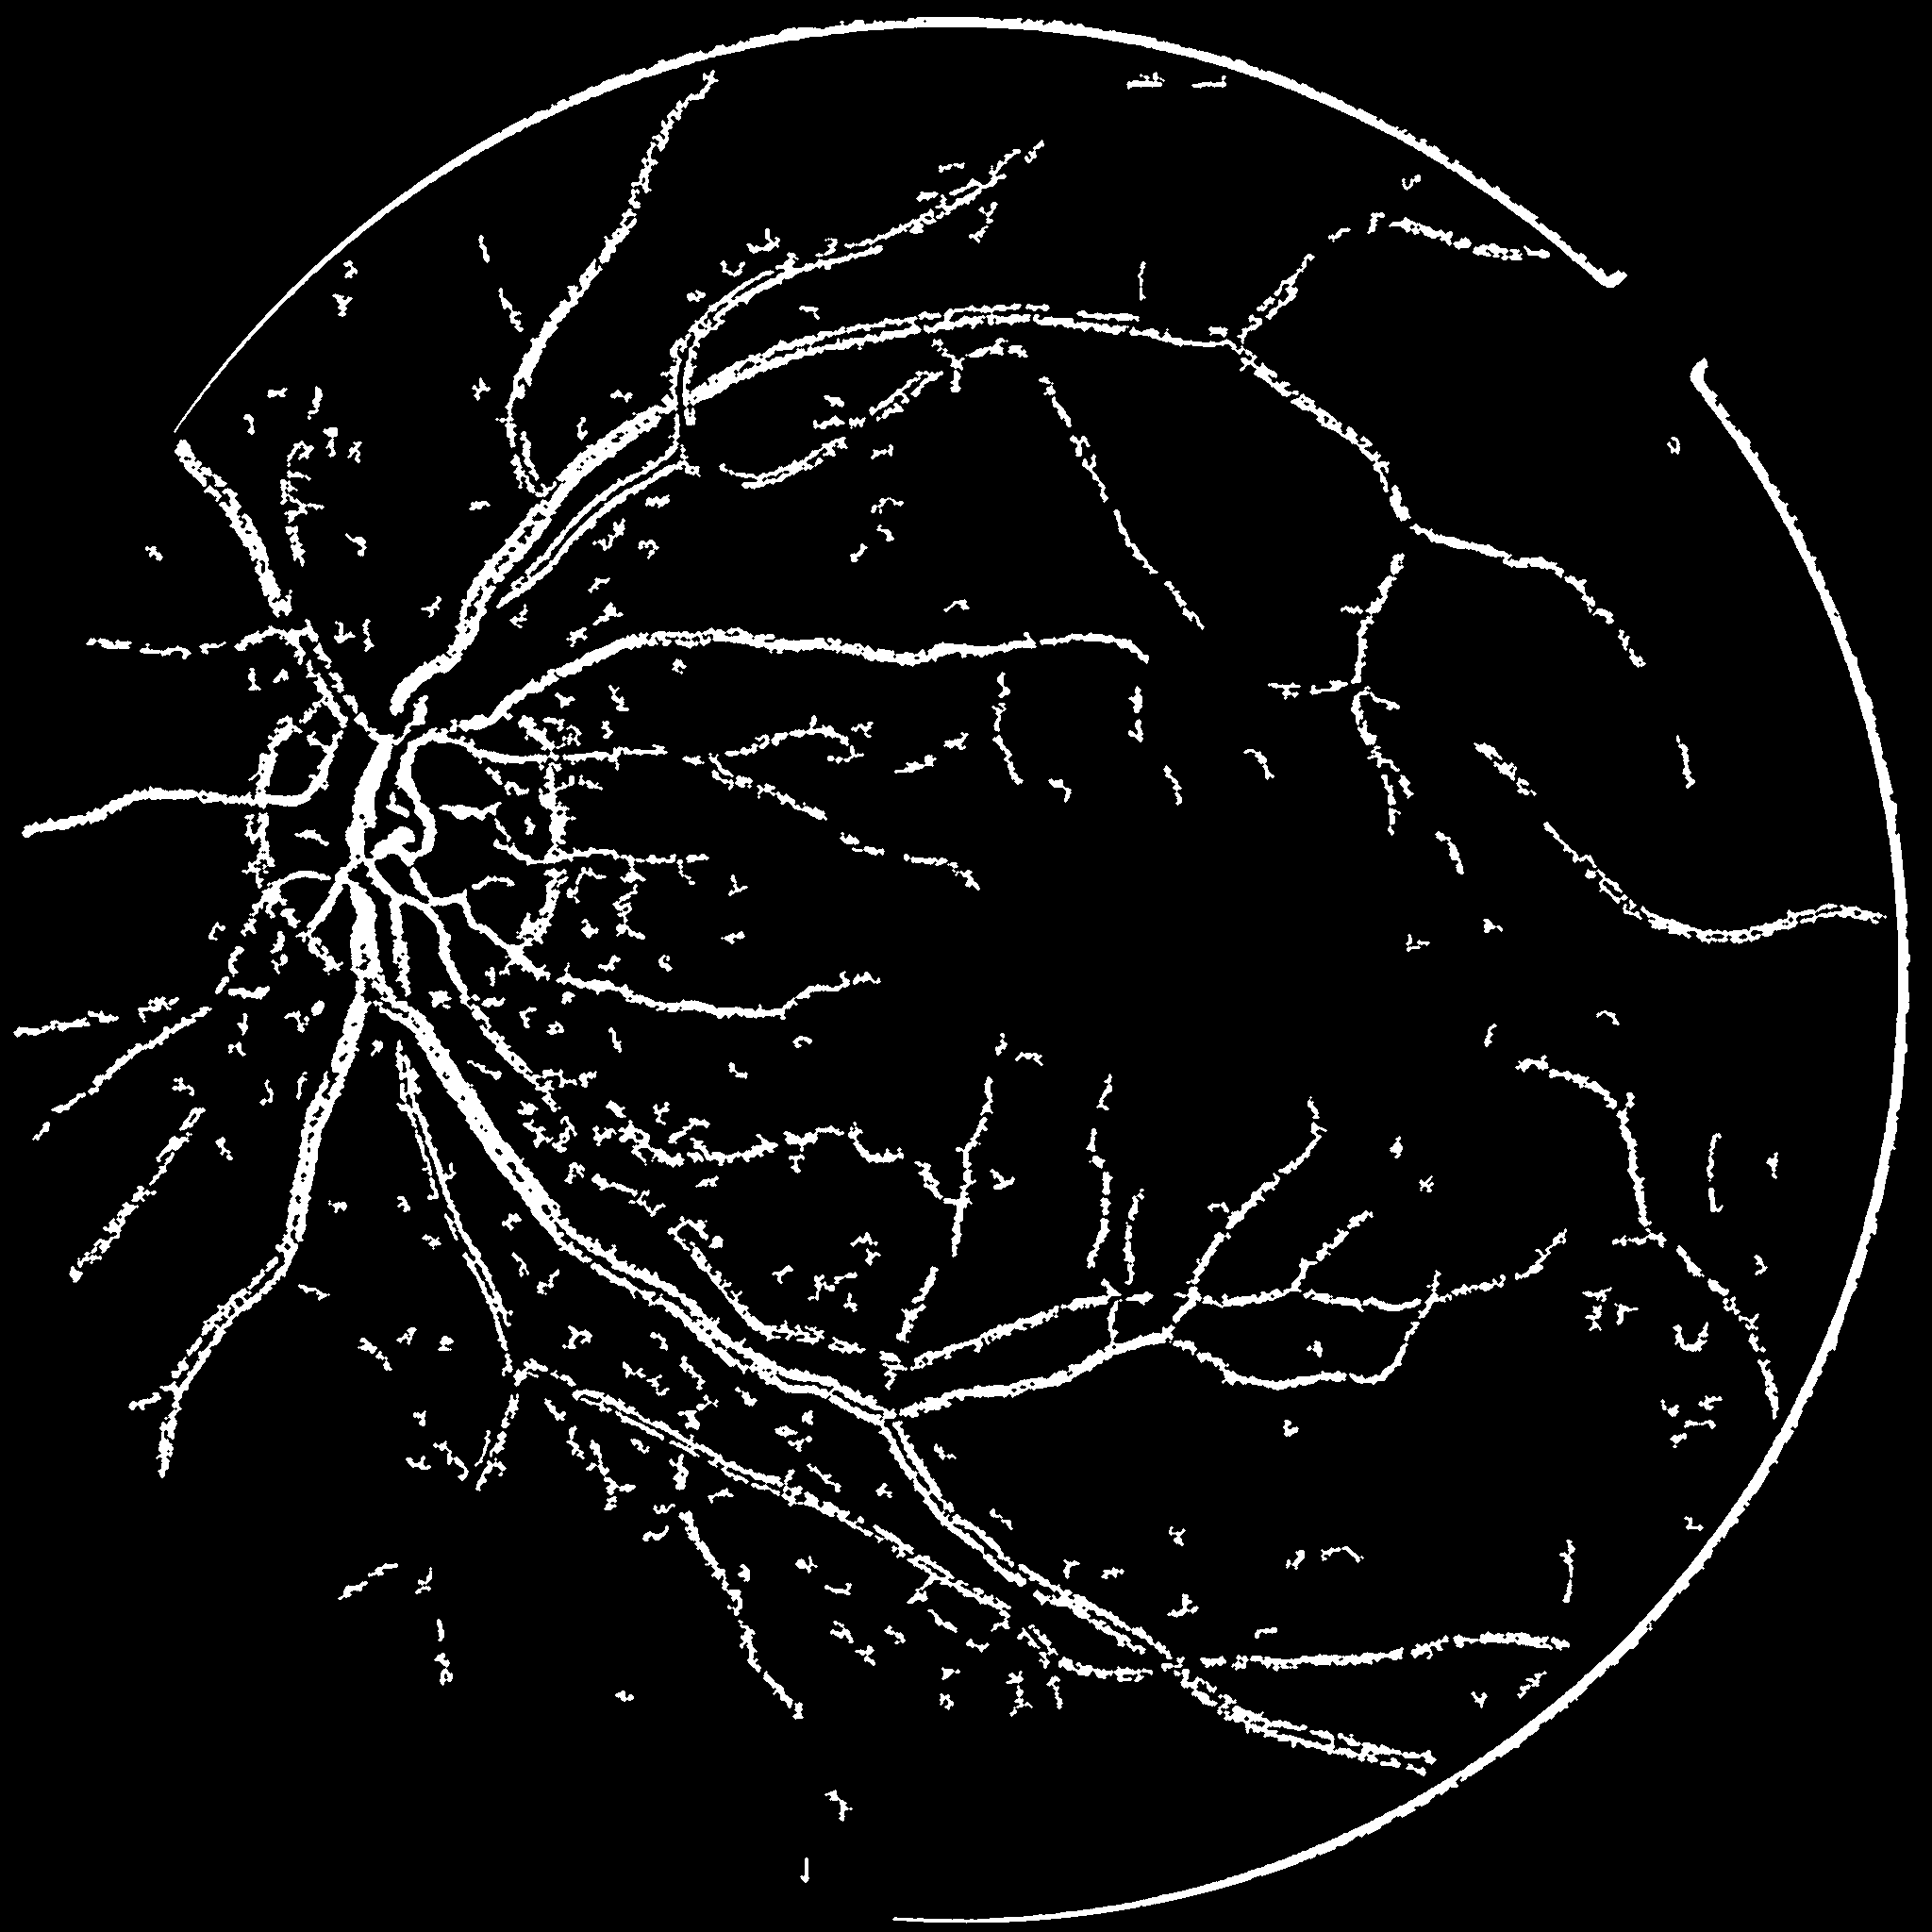
\includegraphics[width=0.28\textwidth]{results/3_A.png} &

\includegraphics[width=0.28\textwidth]{validation_set/masks/3_A.png} \\[10pt]


\includegraphics[width=0.28\textwidth]{training_set/images/4_A.png} &
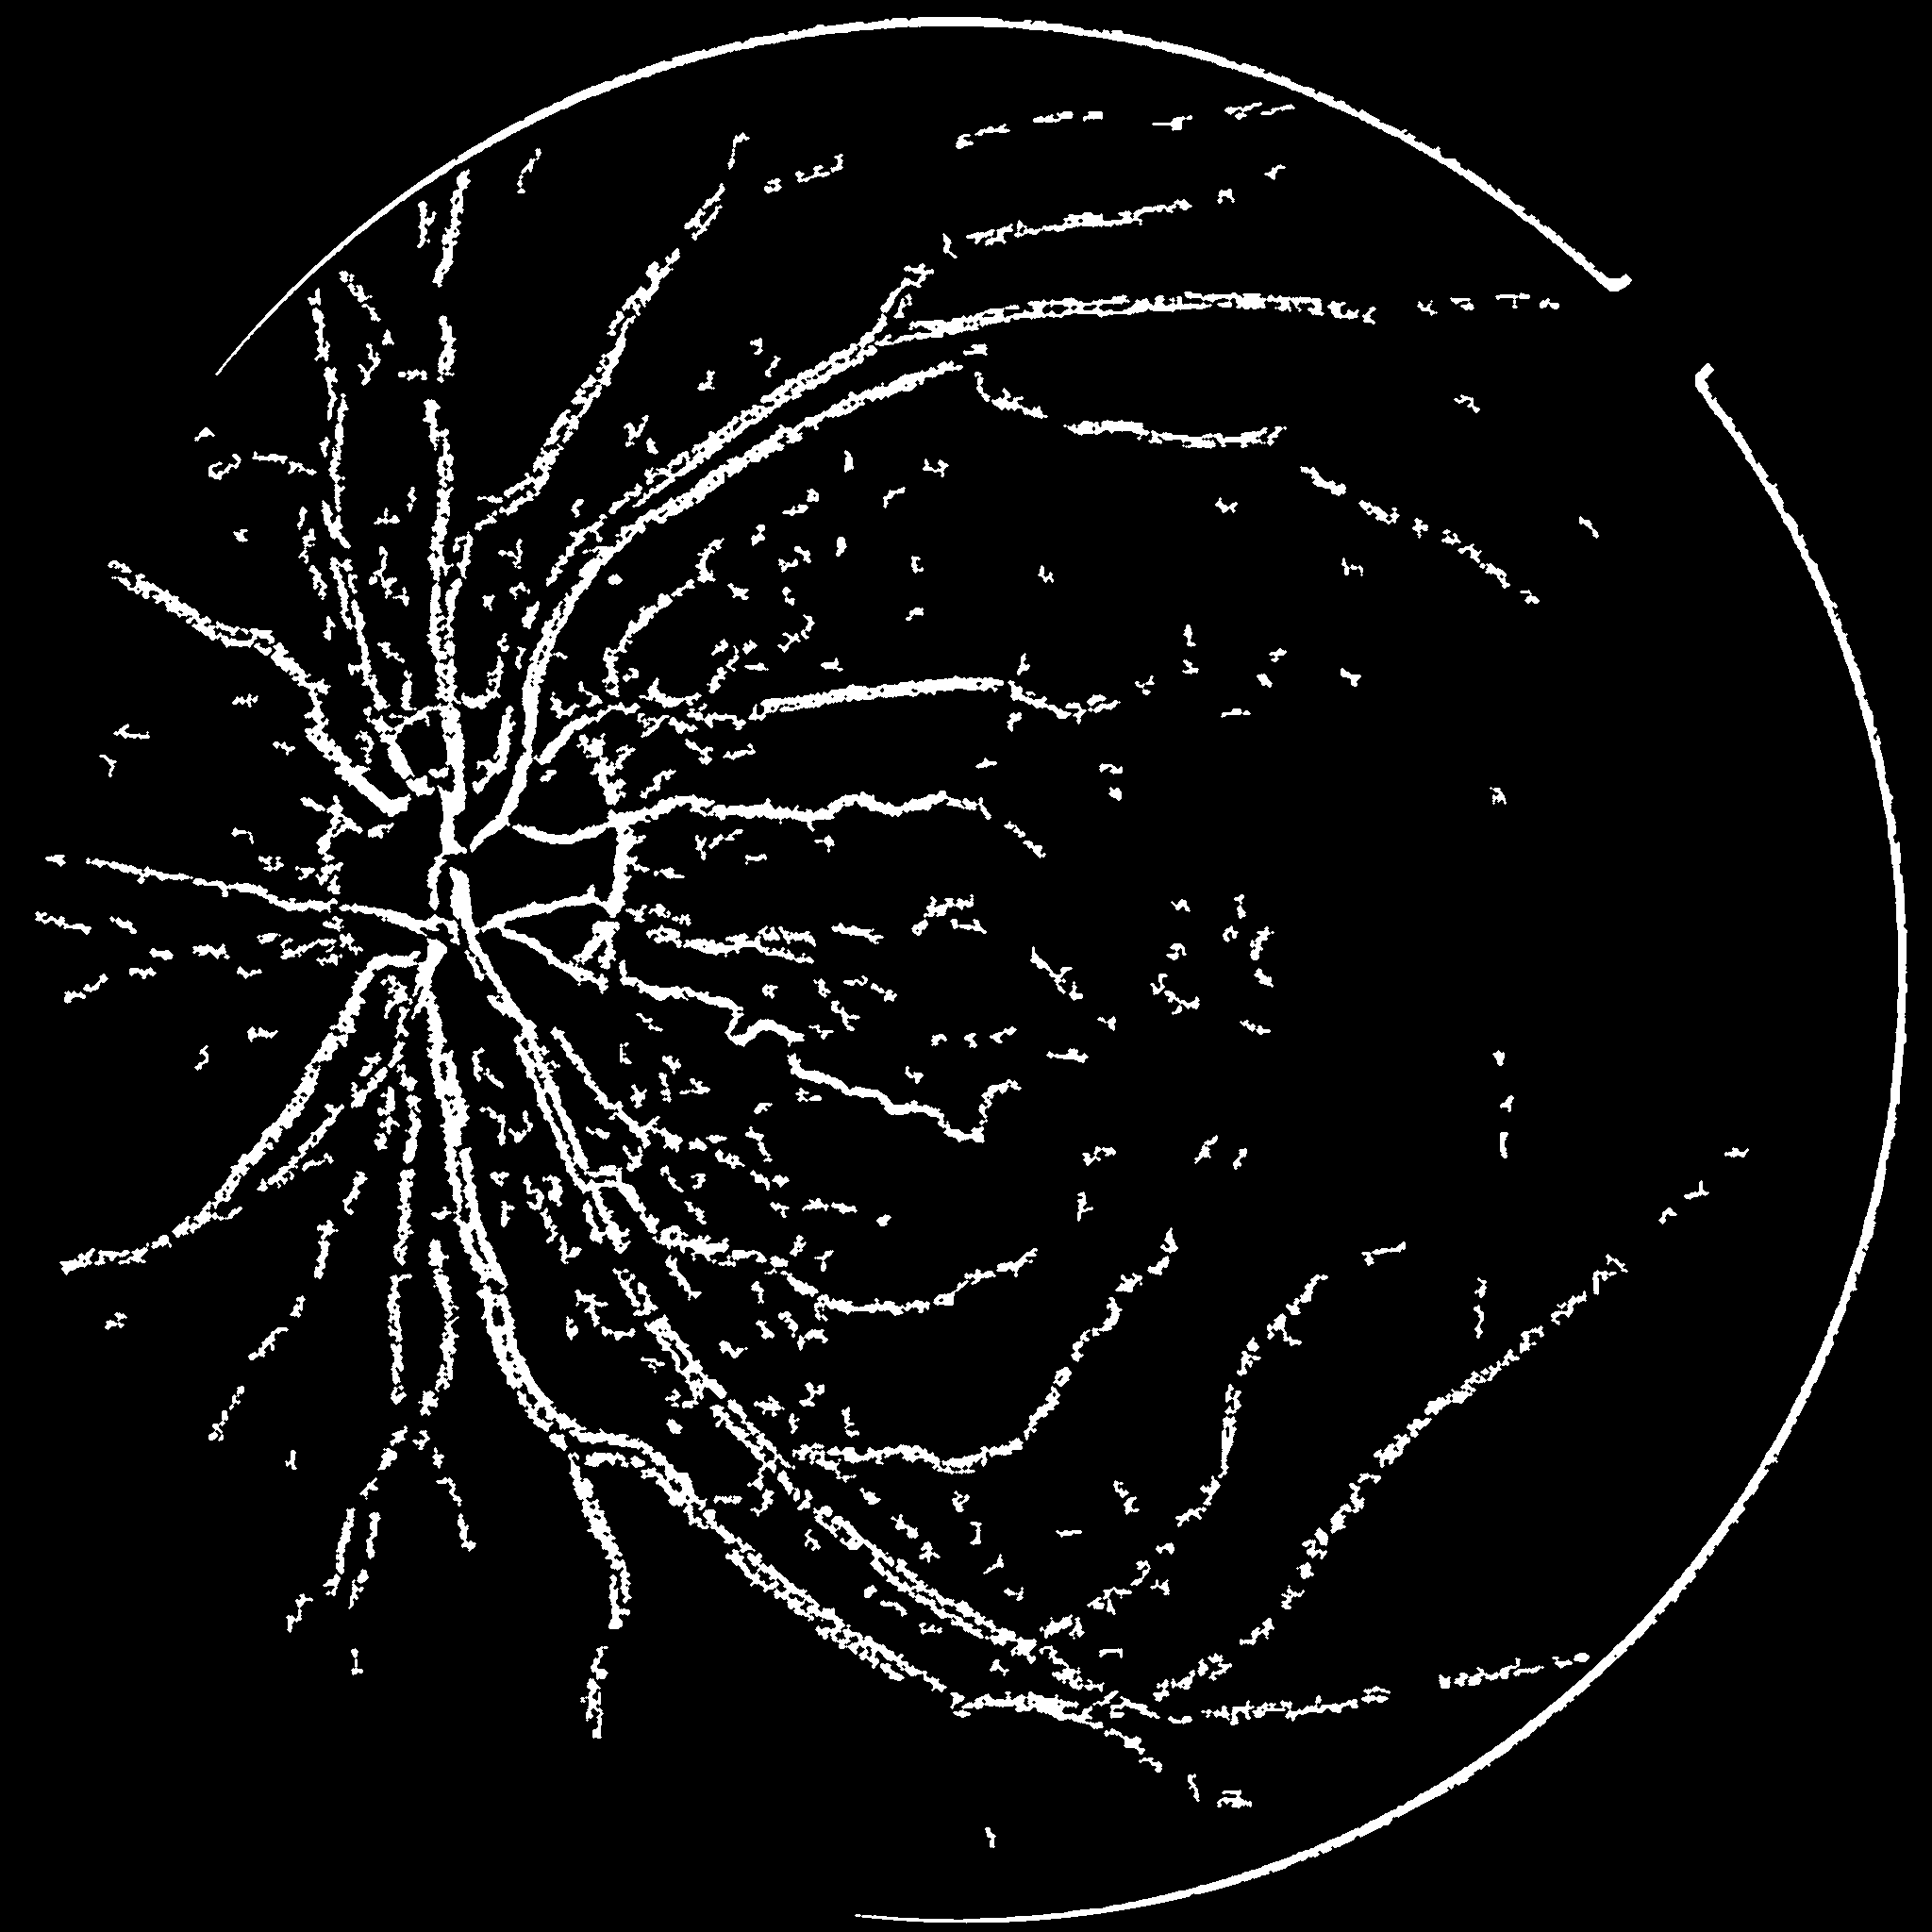
\includegraphics[width=0.28\textwidth]{results/4_A.png} &

\includegraphics[width=0.28\textwidth]{validation_set/masks/4_A.png} \\[10pt]


\includegraphics[width=0.28\textwidth]{training_set/images/5_A.png} &
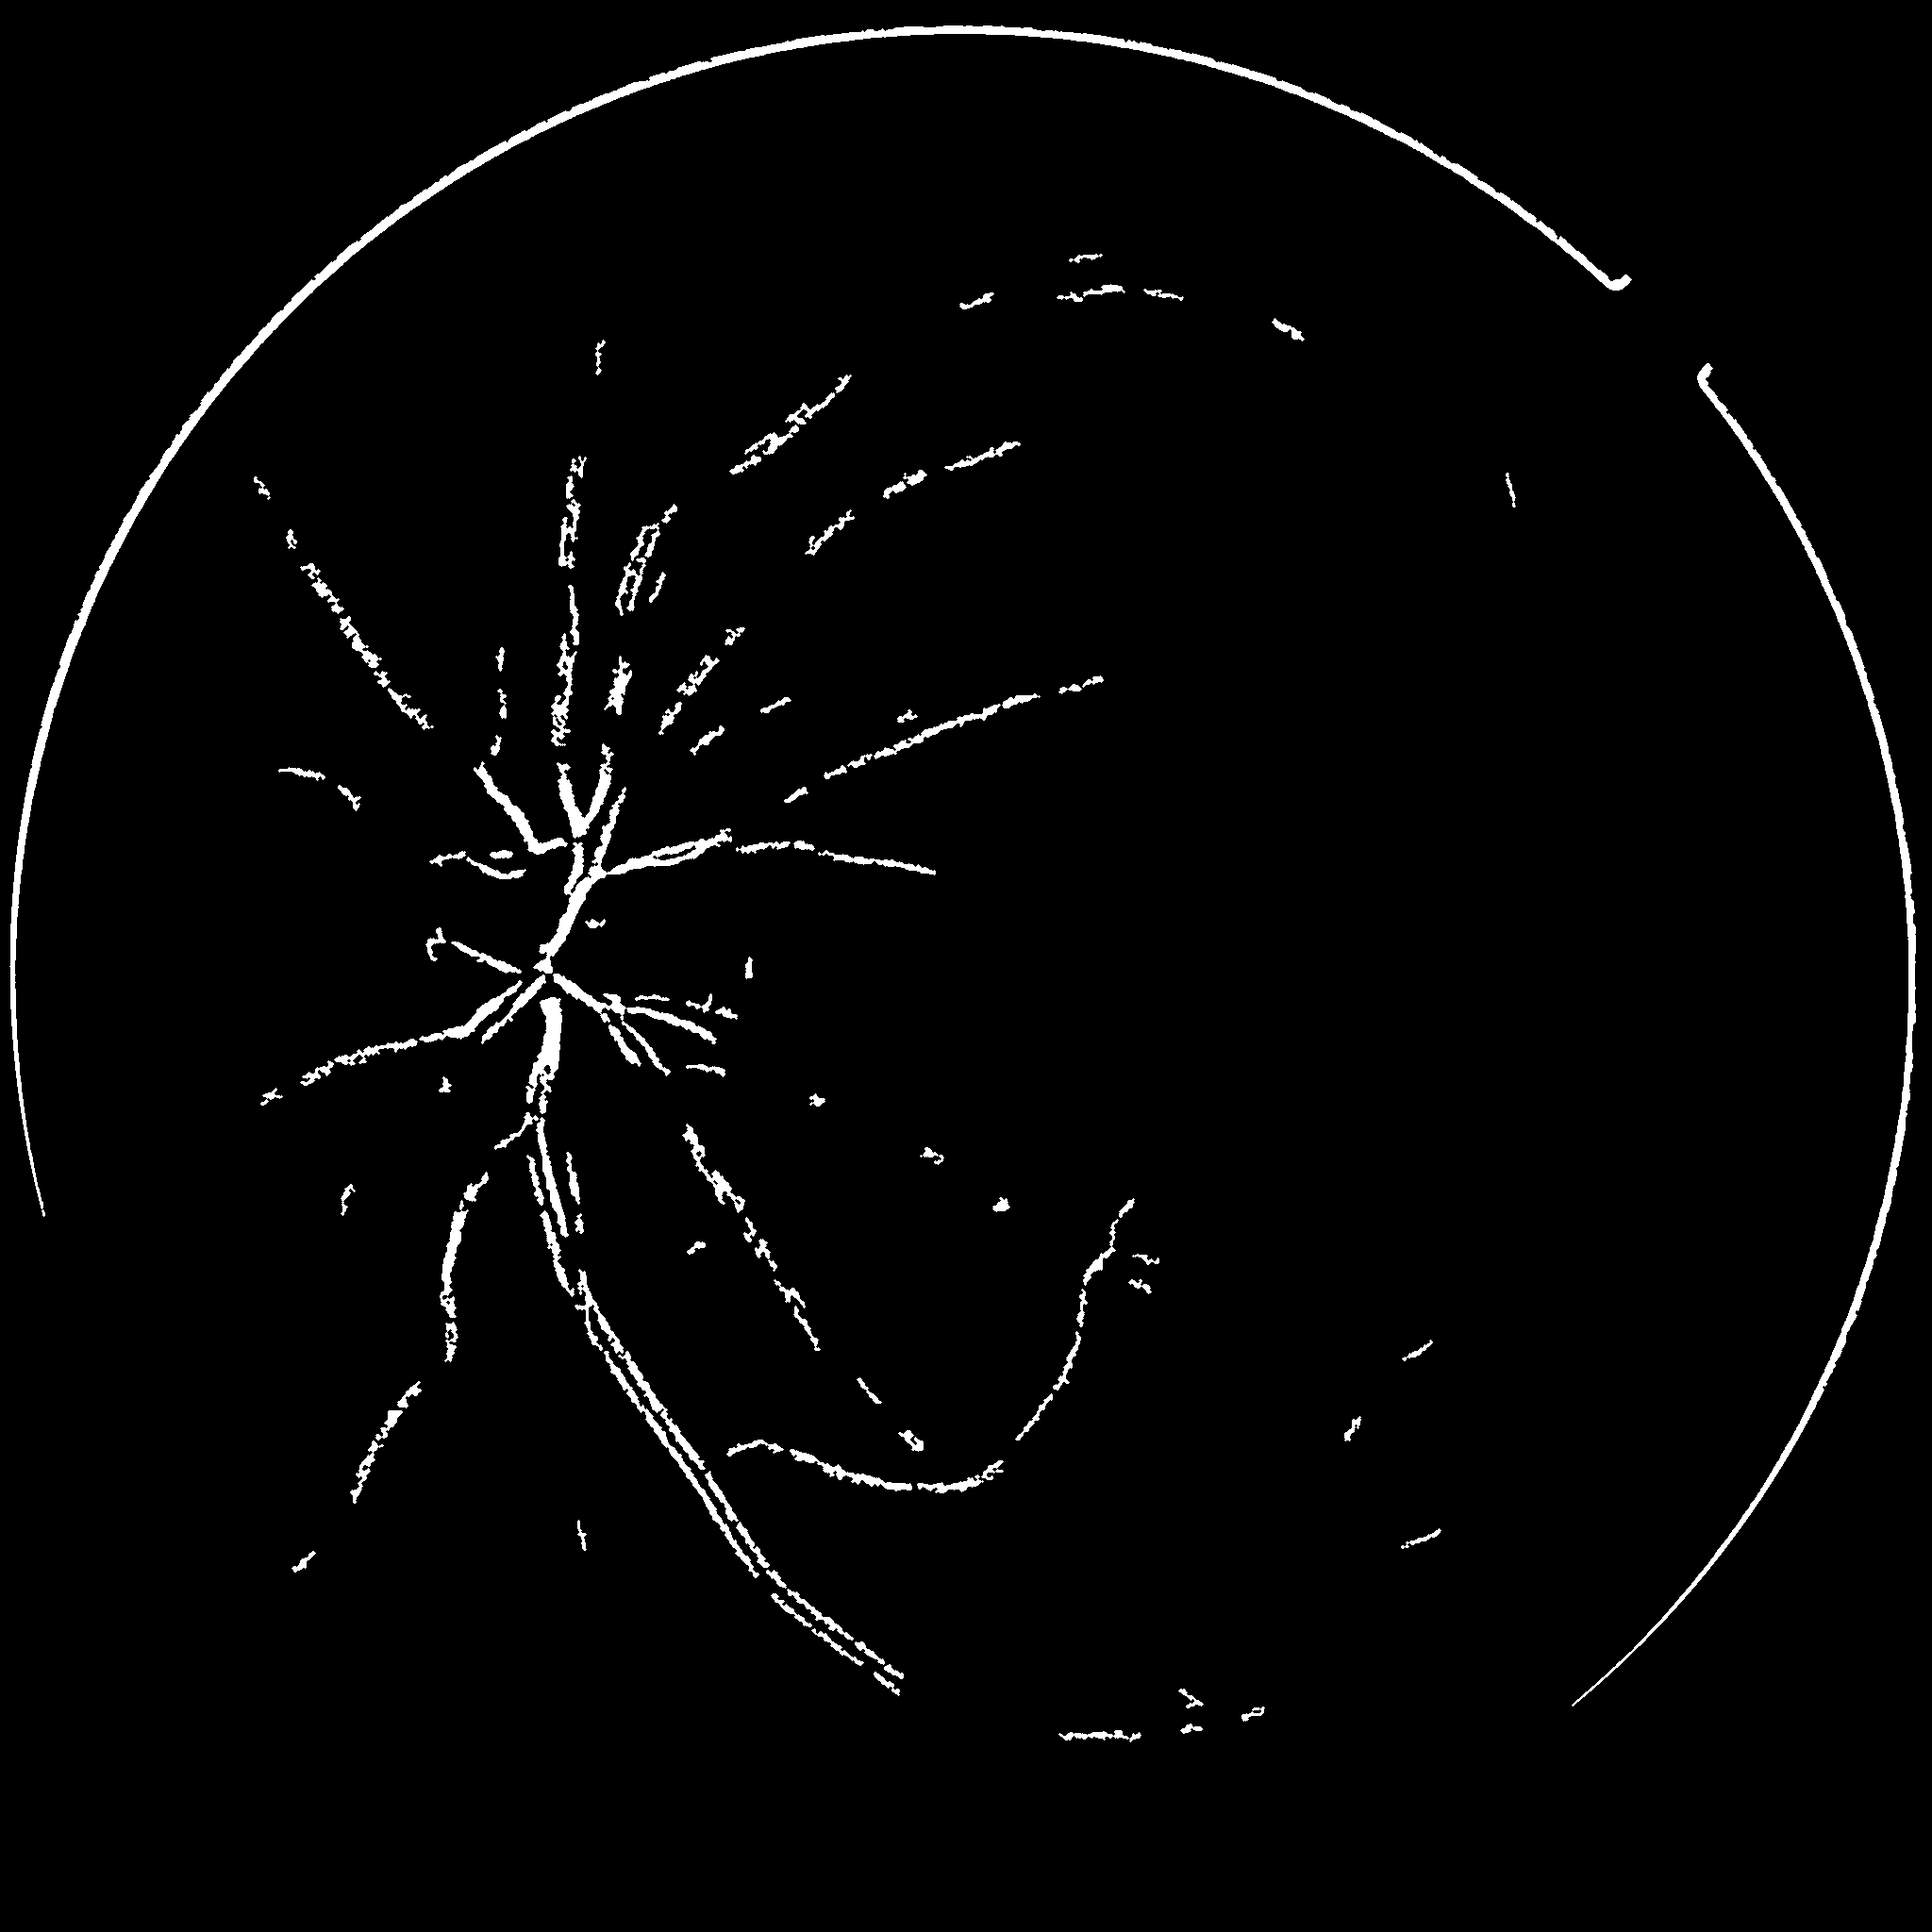
\includegraphics[width=0.28\textwidth]{results/5_A.png} &

\includegraphics[width=0.28\textwidth]{validation_set/masks/5_A.png} \\[10pt]


\includegraphics[width=0.28\textwidth]{training_set/images/6_A.png} &
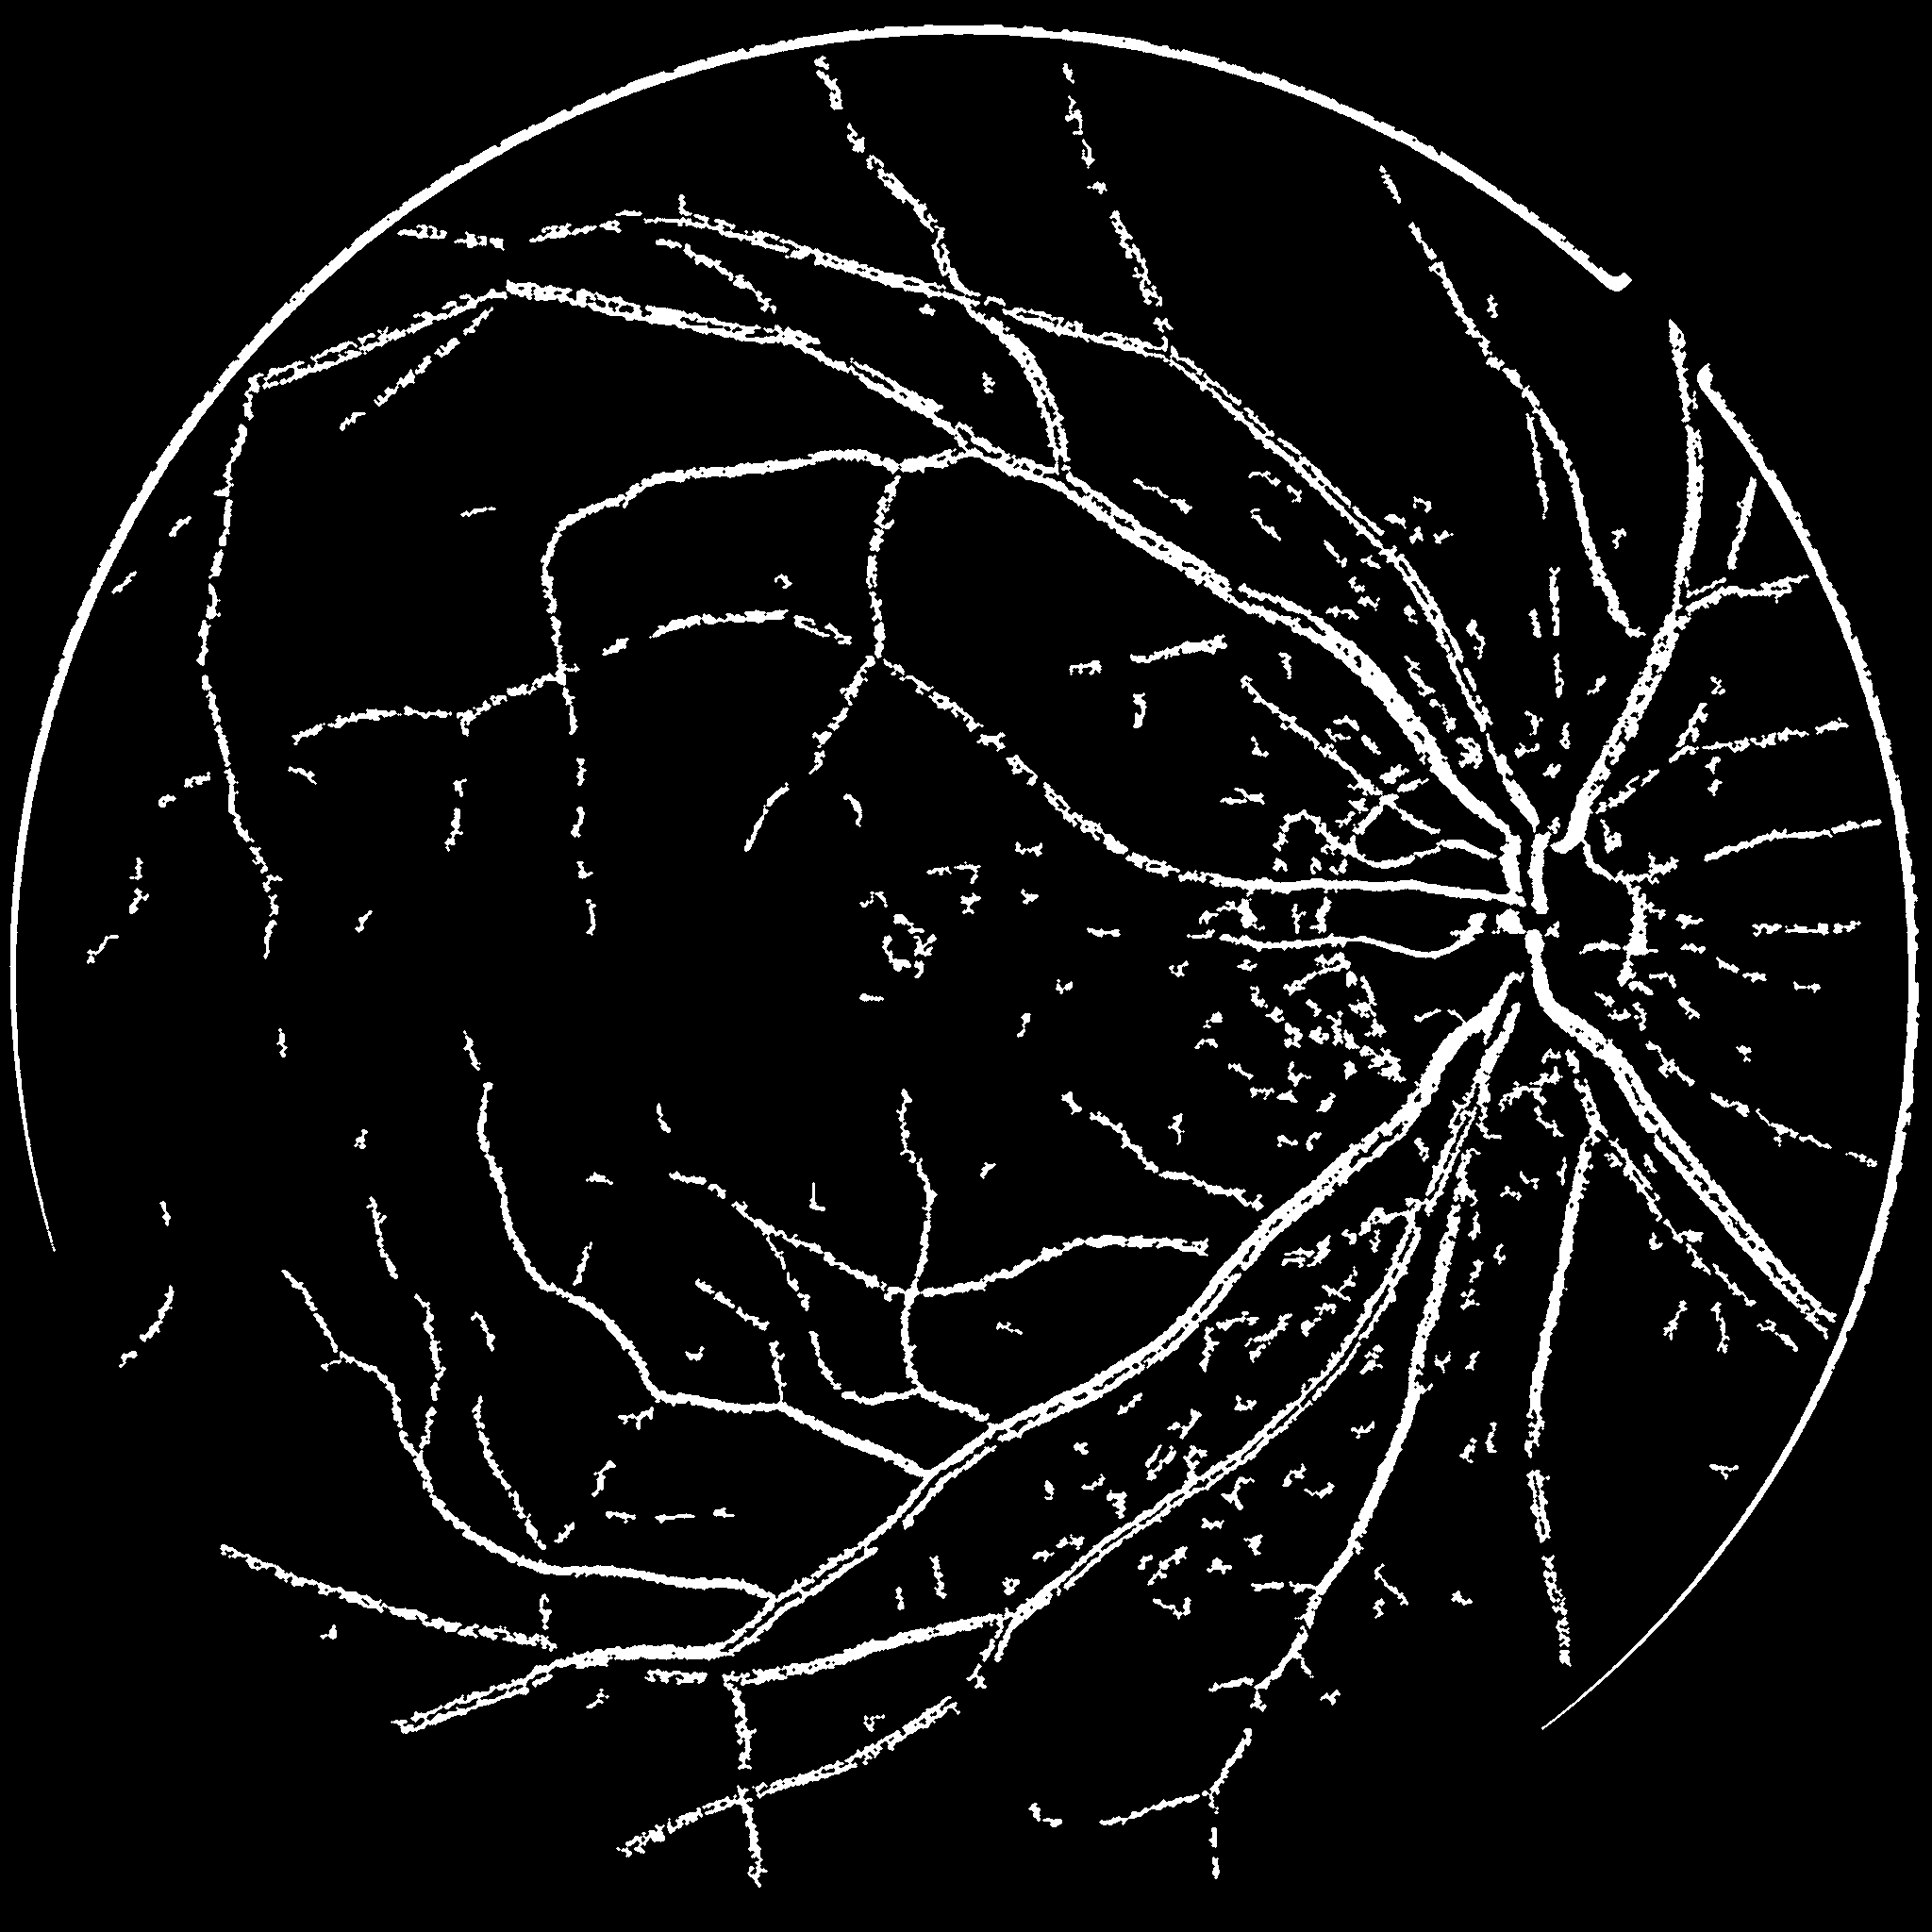
\includegraphics[width=0.28\textwidth]{results/6_A.png} &

\includegraphics[width=0.28\textwidth]{validation_set/masks/6_A.png} \\[10pt]


\includegraphics[width=0.28\textwidth]{training_set/images/7_A.png} &
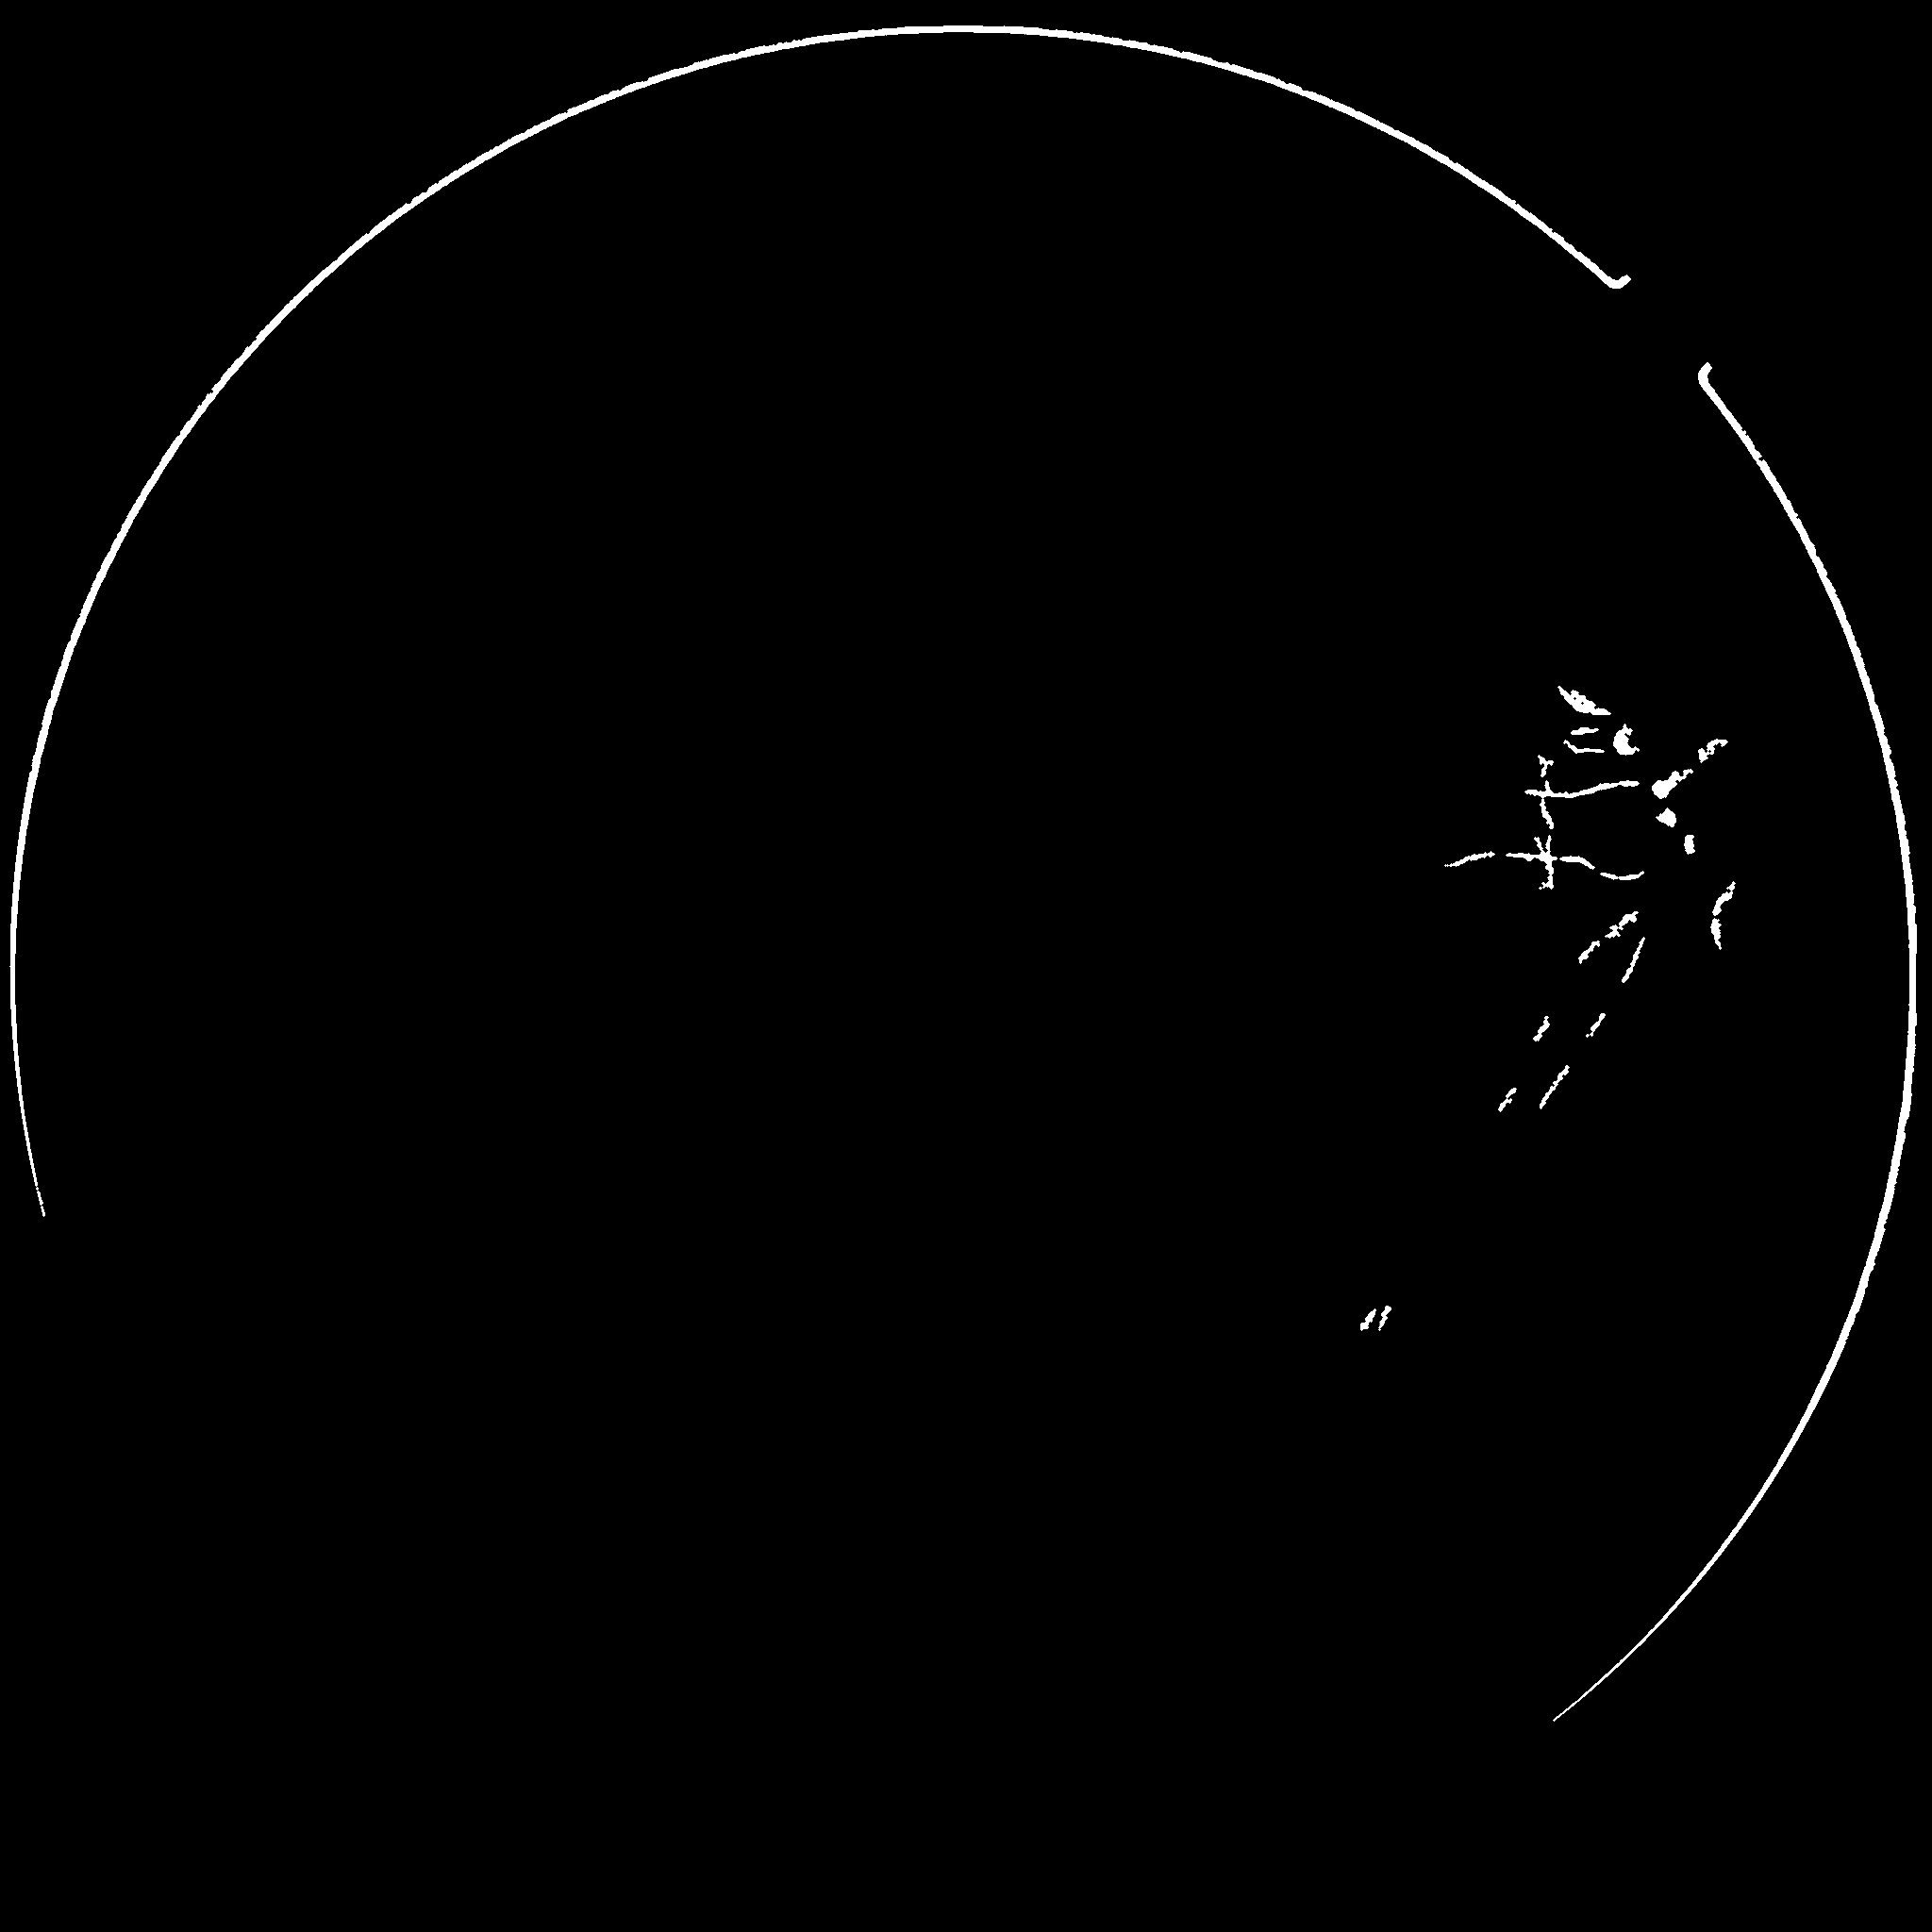
\includegraphics[width=0.28\textwidth]{results/7_A.png} &

\includegraphics[width=0.28\textwidth]{validation_set/masks/7_A.png} \\[10pt]


\includegraphics[width=0.28\textwidth]{training_set/images/8_A.png} &
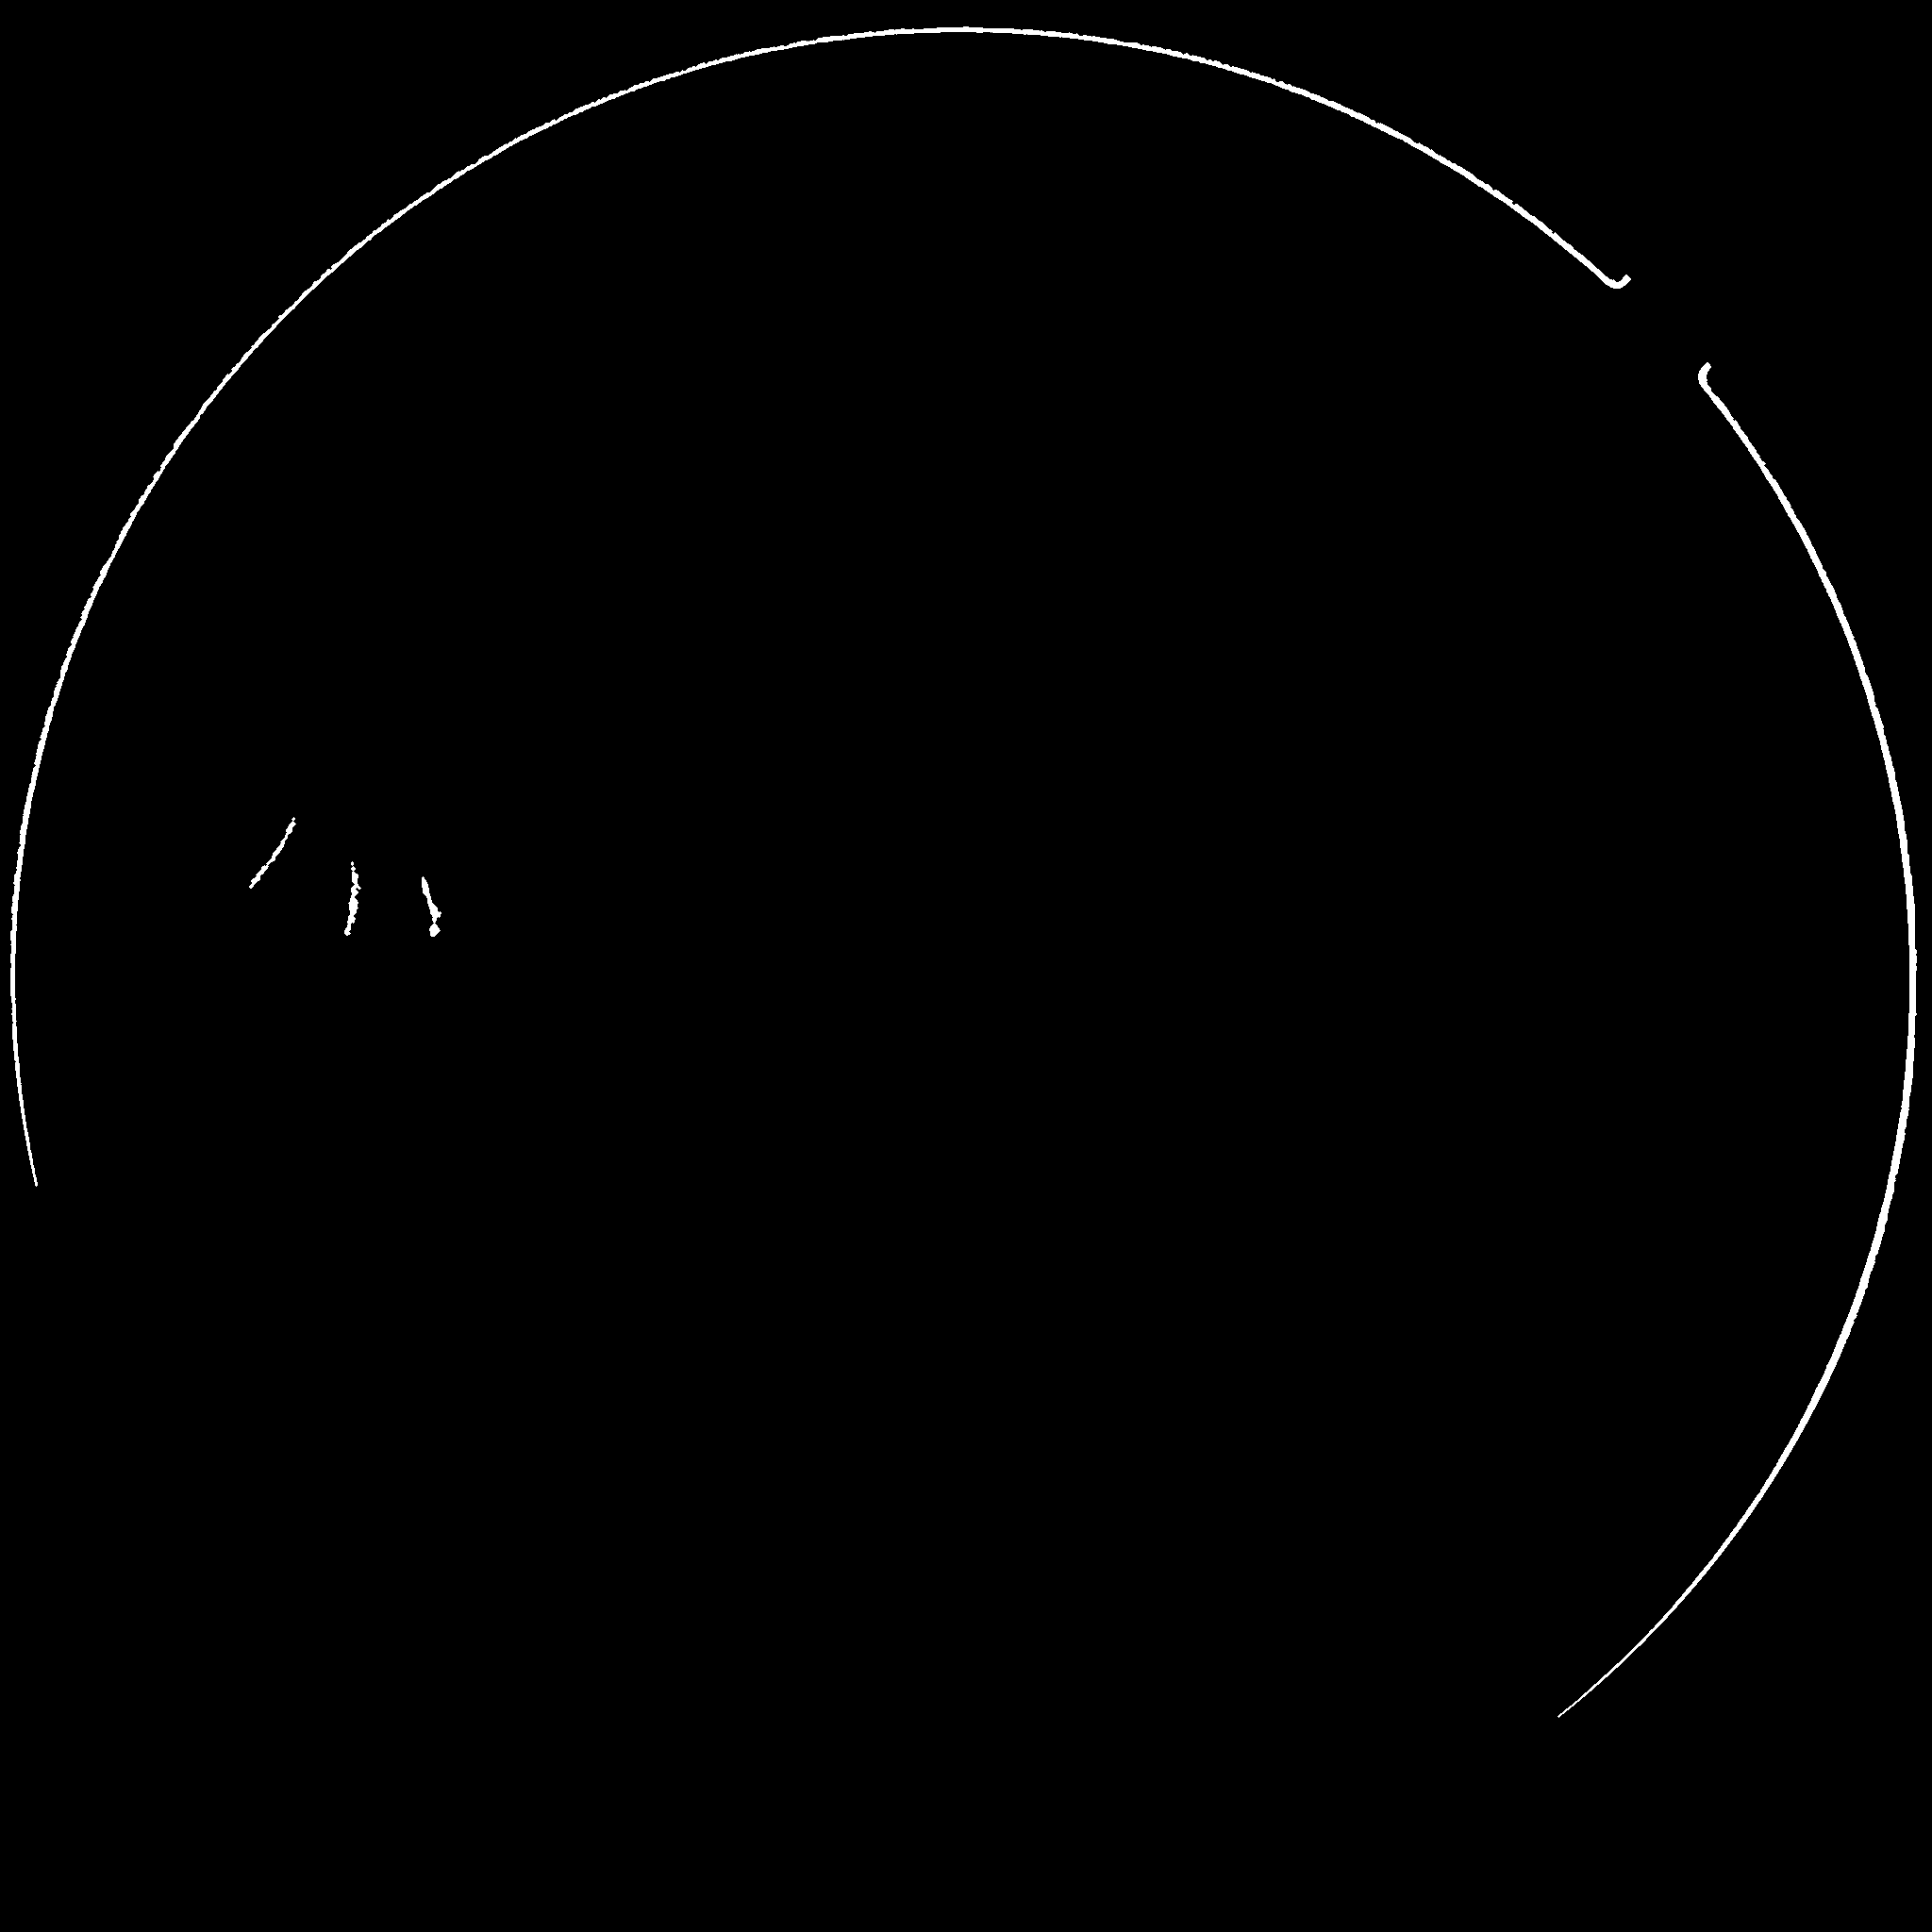
\includegraphics[width=0.28\textwidth]{results/8_A.png} &

\includegraphics[width=0.28\textwidth]{validation_set/masks/8_A.png} \\[10pt]


\includegraphics[width=0.28\textwidth]{training_set/images/9_A.png} &
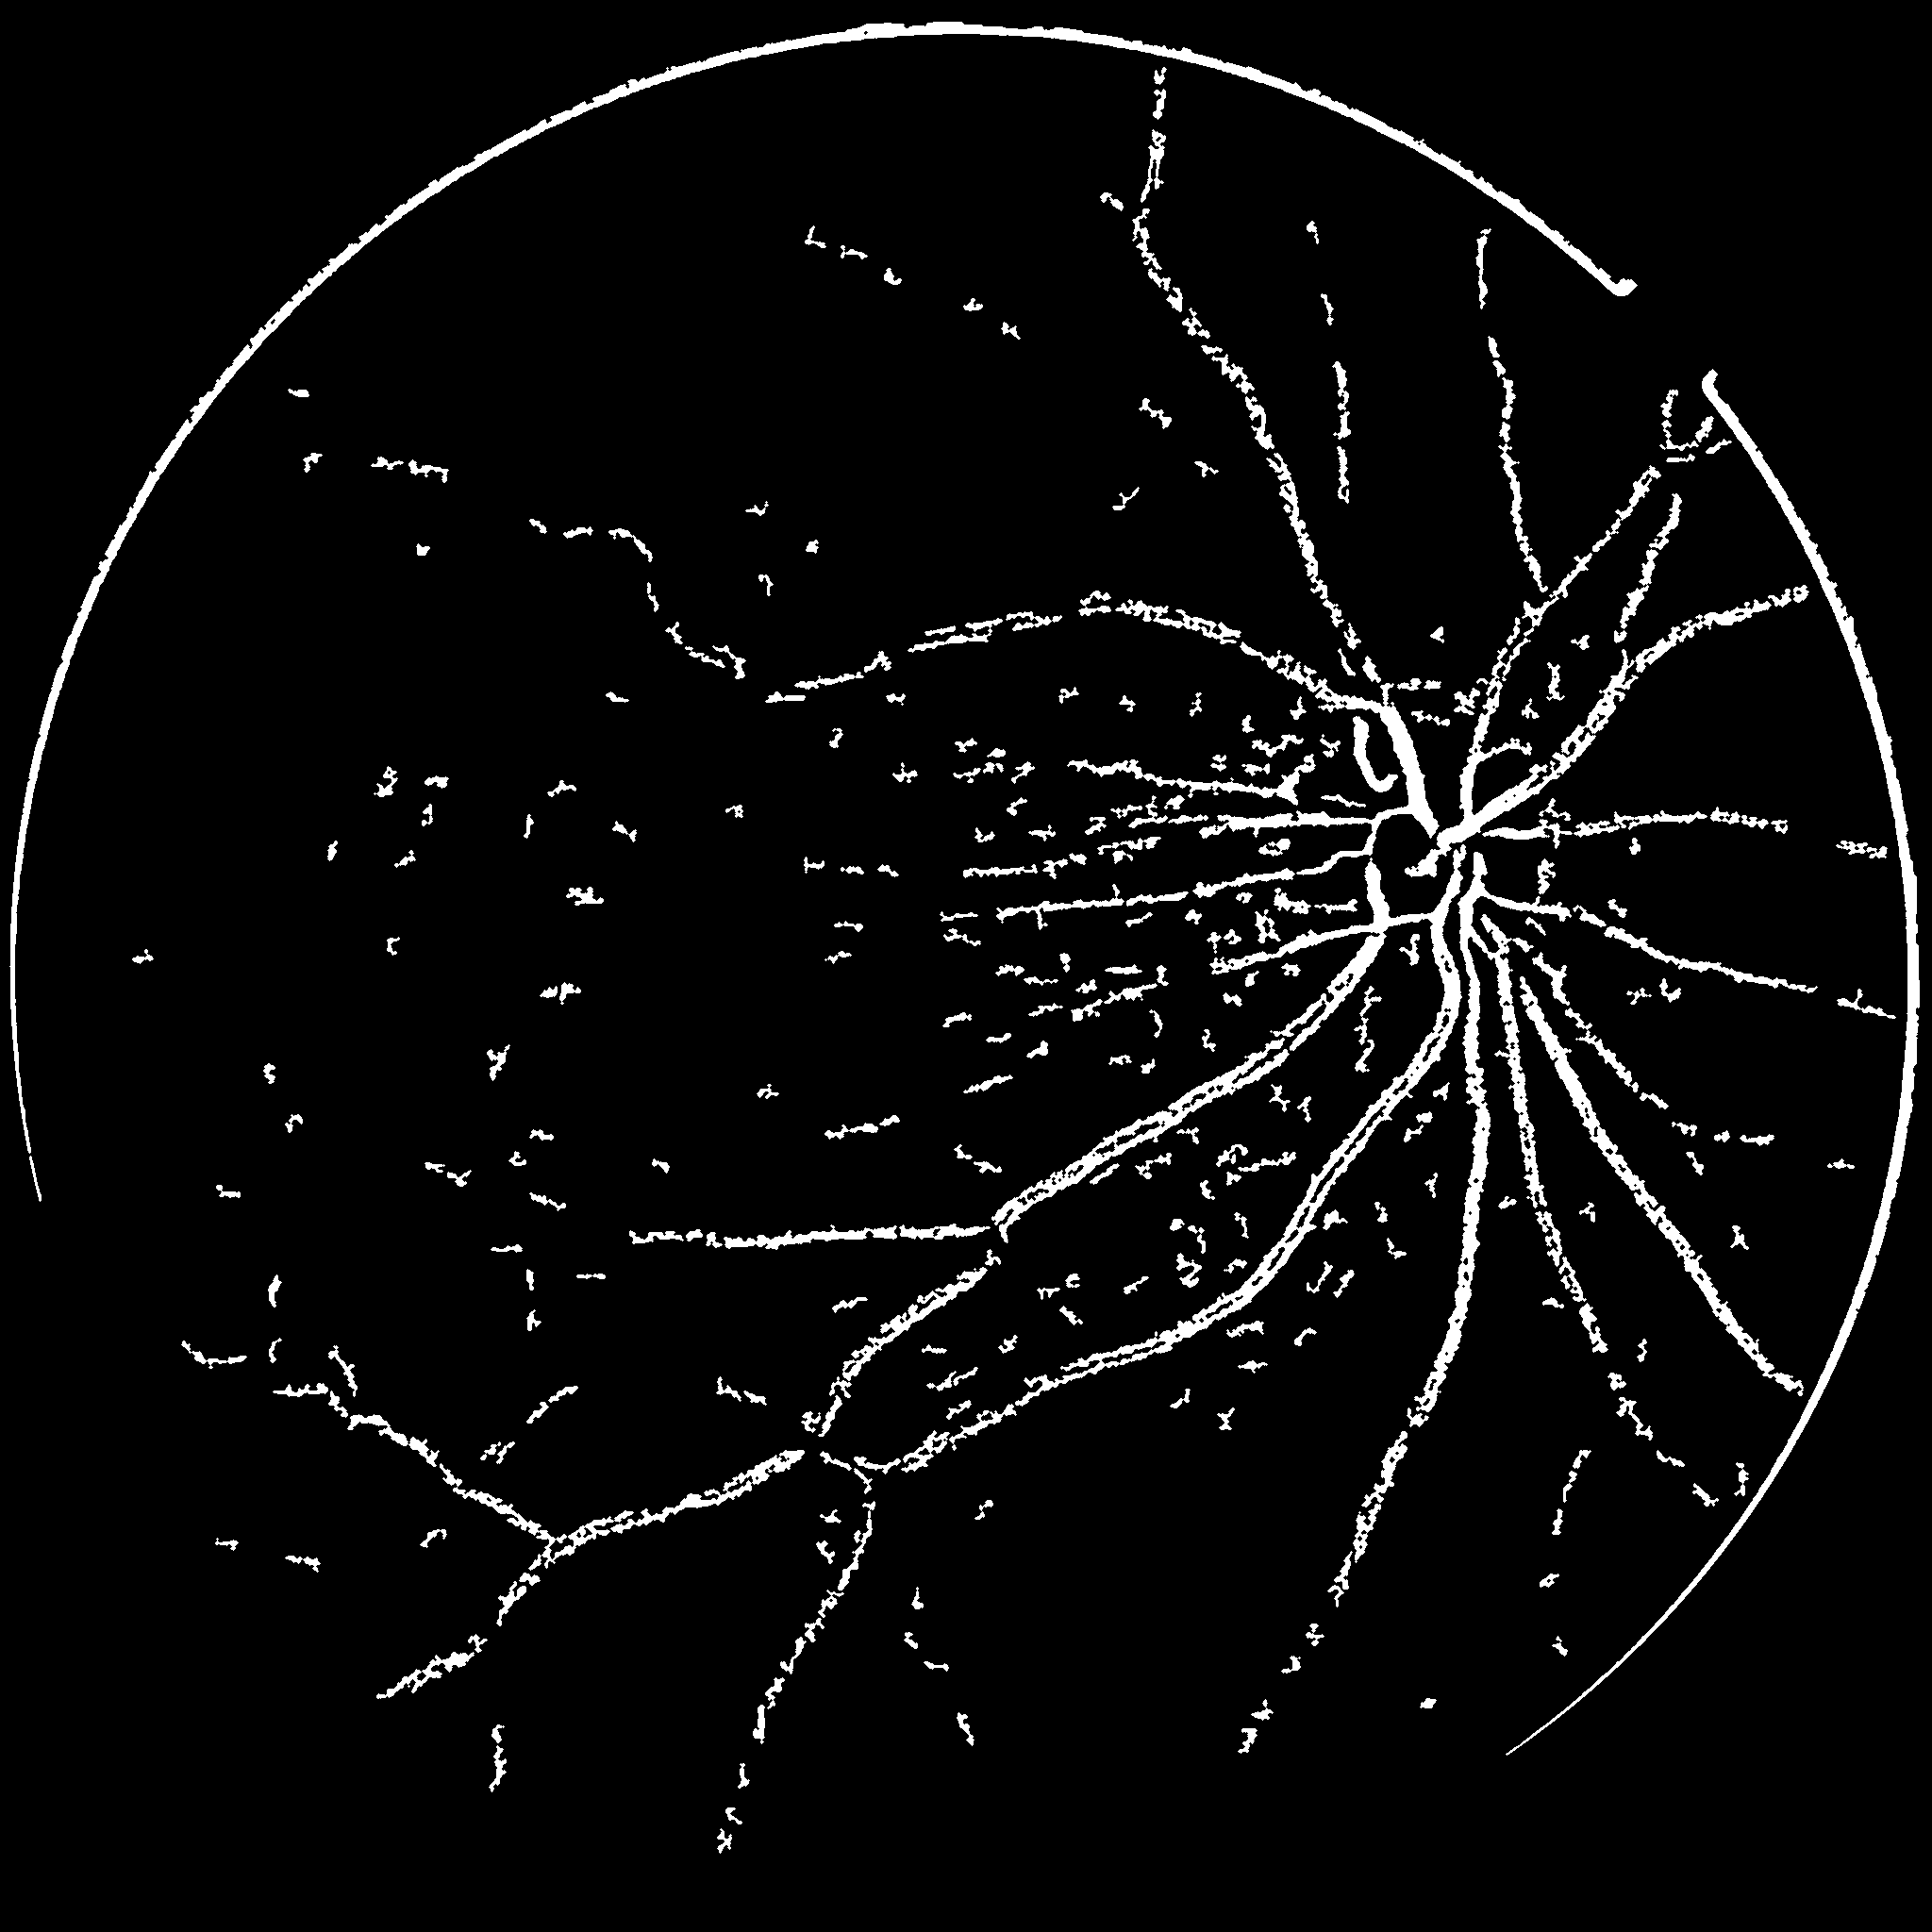
\includegraphics[width=0.28\textwidth]{results/9_A.png} &

\includegraphics[width=0.28\textwidth]{validation_set/masks/9_A.png} \\[10pt]


\includegraphics[width=0.28\textwidth]{training_set/images/10_A.png} &
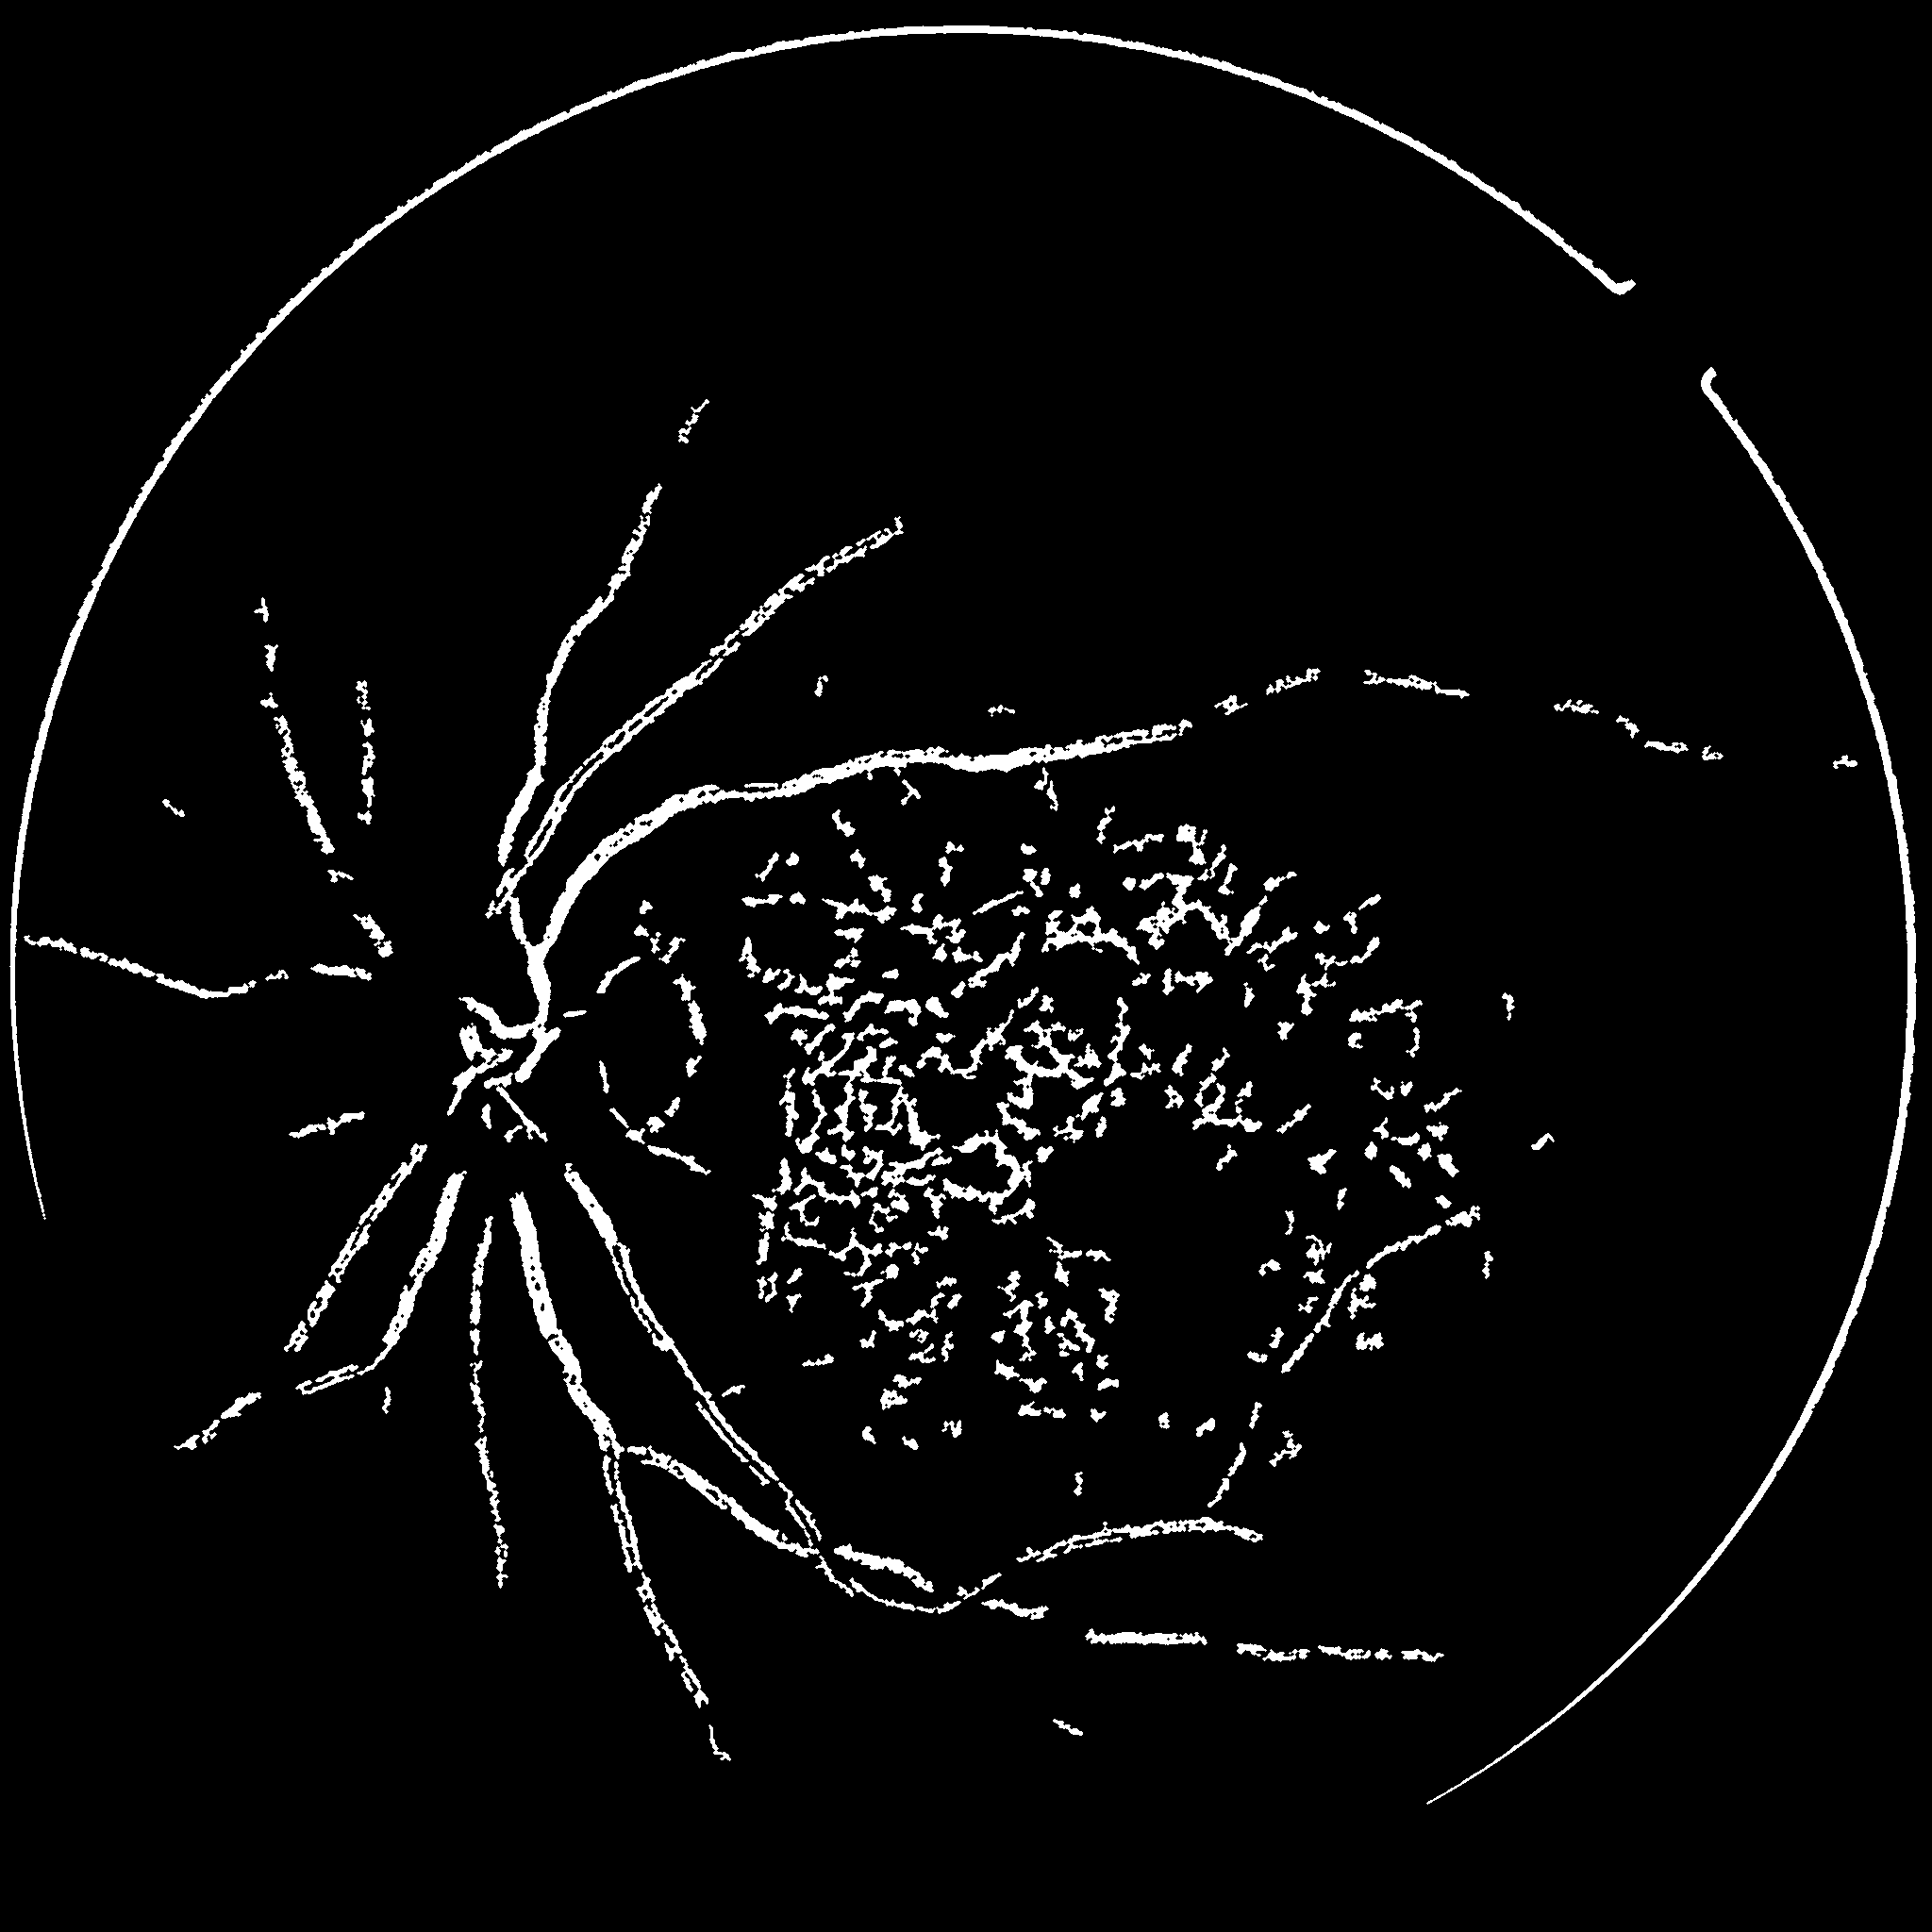
\includegraphics[width=0.28\textwidth]{results/10_A.png} &

\includegraphics[width=0.28\textwidth]{validation_set/masks/10_A.png} \\

\end{tabular}
\caption{Comparison of original fundus images, segmented outputs, and corresponding ground truth masks for 10 representative test cases}
\label{fig:results_vs_gt}
\end{figure}

\hyperref[contents]{\small Back to Table of Contents}
\newpage

\section*{Results}

The segmentation algorithm was evaluated on 200 training images using grid search to determine optimal parameters. The best performance was achieved using:

\begin{itemize}
\item Gaussian Kernel Size = 61
\item Global Threshold (T) = 8
\item Dilation Iterations = 2
\end{itemize}

The optimized parameters were validated on a 50 image annotated subset. Performance metrics are summarized in Table~\ref{tab:segmentation_results}.

\begin{table}[H]
\centering
\begin{tabular}{|c|c|c|}
\hline
\textbf{Dataset} & \textbf{Dice} & \textbf{Jaccard} \\
\hline
Training Set (200 images) & 0.3123 & 0.1979 \\
Validation Set (50 images) & 0.5041 & 0.3440 \\
\hline
\end{tabular}
\caption{Average segmentation performance}
\label{tab:segmentation_results}
\end{table}

\hyperref[contents]{\small Back to Table of Contents}
\newpage

\section*{Discussion}

The proposed classical segmentation pipeline achieved a validation Dice score of 0.504 and Jaccard index of 0.344, indicating moderate agreement with expert annotated vessel masks. Illumination correction significantly improved vessel contrast, while low global thresholding preserved thin capillaries. Morphological dilation and closing enhanced structural continuity. Although classical threshold based methods are sensitive to intensity variations, the results demonstrate that carefully designed traditional image processing techniques can achieve reliable vessel segmentation without using AI or deep learning methods.



\bibliographystyle{ieeetr} 
\bibliography{references}
Add the references if any.


\end{document}